\documentclass[12pt]{article}% Your documentclass. I recommend something from the KOMA script class

%------------------------------------------%
%                Packages
%------------------------------------------%
%------------------------------------------%
%                Packages
%------------------------------------------%

%------------------------------------------%
% Text encoding and layout
%------------------------------------------%

\usepackage[utf8]{inputenx}     % Proper input encoding (UTF-8)
\usepackage{ragged2e}           % Improved text alignment tools
\usepackage{setspace}           % Control line spacing (single, double, etc.)
\usepackage[
  paperwidth=8.5in,
  paperheight=11in,
  margin=1in
]{geometry}                     % Page dimensions and margins

%------------------------------------------%
% Graphics and float control
%------------------------------------------%

\usepackage{graphicx}           % Include graphics
\usepackage{grffile}            % Support graphics with multiple dots in filename
\usepackage{float}              % Improved float placement control
\usepackage{morefloats}         % Increase number of allowed floats
\usepackage{placeins}           % \FloatBarrier to keep floats within sections
\usepackage{pdflscape}          % Landscape pages in PDF
\usepackage{everypage}          % Page number control for rotated pages

%------------------------------------------%
% Mathematics
%------------------------------------------%

\usepackage{amsmath, amssymb, mathrsfs,bbold} % Core math packages
\usepackage{bm}                        % Bold math symbols
\usepackage{accents}                   % Custom math accents

%------------------------------------------%
% Tables
%------------------------------------------%

\usepackage{booktabs}        % Professional-quality tables
\usepackage{threeparttable}  % Tables with notes below
\usepackage{rotating}        % Sideways tables
\usepackage{adjustbox}       % Resize tables/figures relative to text width
\usepackage{siunitx}         % Align numbers by decimal; handle units
\usepackage{longtable}       % Multi-page tables (kableExtra longtable output)
\usepackage{multirow}        % Multi-row cells (kableExtra collapse_rows)
\usepackage{makecell}        % Line breaks inside cells

\sisetup{
  detect-mode,
  group-digits           = false,
  input-symbols          = {( ) [ ] - +},
  table-align-text-post  = false,
  input-signs            = ,
  separate-uncertainty   = true
}

%------------------------------------------%
% Captions and subfigures
%------------------------------------------%

\usepackage{caption}
\usepackage[list=true]{subcaption}
\captionsetup[table]{position=top}
\captionsetup[figure]{position=bottom}

%------------------------------------------%
% Colors and text utilities
%------------------------------------------%

\usepackage{xcolor}     % Extended color support
\usepackage{soul}       % Highlighting and letter spacing
\usepackage{comment}    % Block comments

%------------------------------------------%
% Appendix formatting
%------------------------------------------%

\usepackage[titletoc]{appendix}  % Appendix control and ToC integration

%------------------------------------------%
% Bibliography
%------------------------------------------%

\usepackage{natbib}     % Author-year citation management

%------------------------------------------%
% Hyperlinks (load near the end)
%------------------------------------------%

\usepackage[
  breaklinks,
  colorlinks,
  linkcolor=black,
  citecolor=black,
  urlcolor=blue,
  hyperfootnotes=false
]{hyperref}

% Allow URL line breaks at many characters
\def\UrlBreaks{%
\do\/\do-\do.\do=\do_\do?\do\&\do\%\do\a\do\b\do\c\do\d\do\e\do\f\do\g\do\h%
\do\i\do\j\do\k\do\l\do\m\do\n\do\o\do\p\do\q\do\r\do\s\do\t\do\u\do\v\do\w%
\do\x\do\y\do\z\do\A\do\B\do\C\do\D\do\E\do\F\do\G\do\H\do\I\do\J\do\K\do\L%
\do\M\do\N\do\O\do\P\do\Q\do\R\do\S\do\T\do\U\do\V\do\W\do\X\do\Y\do\Z%
\do\0\do\1\do\2\do\3\do\4\do\5\do\6\do\7\do\8\do\9}

%------------------------------------------%
%              Custom Commands
%------------------------------------------%
%These are the custom commands that I use in the latex document

\newcommand\iid{i.i.d.} %Makes iid a command
\newcommand\pN{\mathcal{N}} %Makes the natural numbers a command


\setcounter{MaxMatrixCols}{20}

\newtheorem{theorem}{Theorem}%[section]
\newtheorem{lemma}[theorem]{Lemma}
\newtheorem{proposition}[theorem]{Proposition}
\newtheorem{corollary}[theorem]{Corollary}
\newtheorem{assumption}[theorem]{Assumption}
\newenvironment{proof}{\paragraph{Proof:}}{\hfill$\square$ \\} %This fixes the problem with dynamic tables for some reason

%For Page Numbers while rotated
\newlength{\hfoot}
\newlength{\vfoot}
\AddEverypageHook{\ifdim\textwidth=\linewidth\relax
\else\setlength{\hfoot}{-\topmargin}%
\addtolength{\hfoot}{-\headheight}%
\addtolength{\hfoot}{-\headsep}%
\addtolength{\hfoot}{-.5\linewidth}%
\ifodd\value{page}\setlength{\vfoot}{\oddsidemargin}%
\else\setlength{\vfoot}{\evensidemargin}\fi%
\addtolength{\vfoot}{\textheight}%
\addtolength{\vfoot}{\footskip}%
\raisebox{\hfoot}[0pt][0pt]{\rlap{\hspace{\vfoot}\rotatebox[origin=cB]{90}{\thepage}}}\fi}
%http://tex.stackexchange.com/questions/209685/landscape-mode-and-page-numbering

%------------------------------------------%
%      Matter Related to Table Creation
%------------------------------------------%
%This helps with custom automatic tables. It uses latex  functions
%http://www.jwe.cc/2012/03/stata-latex-tables-estout/
%http://repec.org/bocode/e/estout/estout.html

% *****************************************************************
% Estout related things
% *****************************************************************
\let\estinput=\input % define a new input command so that we can still flatten the document

\newcommand{\estwide}[3]{
    \vspace{.75ex}{
      \textsymbols% Note the added command here
      \begin{tabular*}
      {\textwidth}{@{\hskip\tabcolsep\extracolsep\fill}l*{#2}{#3}}
      \toprule
      \estinput{#1}
      \bottomrule
      \addlinespace[.75ex]
      \end{tabular*}
      }
    } 

\newcommand{\estauto}[3]{
    \vspace{.75ex}{
      \textsymbols% Note the added command here
      \begin{tabular}{l*{#2}{#3}}
      \toprule
      \estinput{#1}
      \bottomrule
      \addlinespace[.75ex]
      \end{tabular}
      }
    }

% Allow line breaks with \\ in specialcells
\newcommand{\specialcell}[2][c]{%
    \begin{tabular}[#1]{@{}c@{}}#2\end{tabular}
}
\DeclareUnicodeCharacter{00A0}{ }
% *****************************************************************
% Custom subcaptions
% *****************************************************************
% Note/Source/Text after Tables
% The new approach using threeparttables to generate notes that are the exact width of the table.
\newcommand{\Figtext}[1]{%
  \begin{tablenotes}[para,flushleft]
  \hspace{6pt}
  \hangindent=1.75em
  #1
  \end{tablenotes}
  }
\newcommand{\Fignote}[1]{\Figtext{\emph{Note:~}~#1}}
\newcommand{\Figsource}[1]{\Figtext{\emph{Source:~}~#1}}
\newcommand{\Starnote}{\Figtext{* p $<$ 0.1, ** p $<$ 0.05, *** p $<$ 0.01. Robust standard errors in parentheses.}}% Add significance note with \starnote
% If you are using hyper-ref (recommended), this command must go after all 
% other package inclusions (from the hyperref package documentation).
% The purpose of hyperref is to make the PDF created extensively
% cross-referenced.

\newcommand{\sym}[1]{\rlap{#1}} %Allows for fancy stars in tables that also works in beamer

% Create a function that works for the non-linear symbols
\newcommand{\nlsym}[1]{\rlap{\append{}{*}{#1}}} %Allows for fancy stars in tables that also works in beamer

% Character substitution that prints brackets and the minus symbol in text mode. Thanks to David Carlisle
\def\yyy{%
  \bgroup\uccode`\~\expandafter`\string-%
  \uppercase{\egroup\edef~{\noexpand\text{\llap{\textendash}\relax}}}%
  \mathcode\expandafter`\string-"8000 }

\def\xxxl#1{%
\bgroup\uccode`\~\expandafter`\string#1%
\uppercase{\egroup\edef~{\noexpand\text{\noexpand\llap{\string#1}}}}%
\mathcode\expandafter`\string#1"8000 }

\def\xxxr#1{%
\bgroup\uccode`\~\expandafter`\string#1%
\uppercase{\egroup\edef~{\noexpand\text{\noexpand\rlap{\string#1}}}}%
\mathcode\expandafter`\string#1"8000 }

\def\textsymbols{\xxxl[\xxxr]\xxxl(\xxxr)\yyy}


%Protects against odd minus sign errors within the tables
\catcode`_11
\protected\def \c__siunitx_minus_tl {$-$}
\catcode`_ 8 

%-----------Tables-------------%
% This Section is needed to make the tables work with amsmath. But because of the \( being open and having no match, Sublime Text thinks that everything after it (all text) is in math mode and hence changes the text color. This annoys me so the only ``solution'' is to just place this preamble here. It seems to work still. 
\makeatletter 
\edef\originalbmathcode{%
    \noexpand\mathchardef\noexpand\@tempa\the\mathcode`\(\relax} %\)

\def\resetMathstrut@{%
  \setbox\z@\hbox{%
    \originalbmathcode

    \def\@tempb##1"##2##3{\the\textfont"##3\char"}%
    \expandafter\@tempb\meaning\@tempa \relax
  }%
  \ht\Mathstrutbox@\ht\z@ \dp\Mathstrutbox@\dp\z@
}
\makeatother %./tables.tex:25: LaTeX Error: Bad math environment delimiter. [\)]
\usepackage{xparse}

\ExplSyntaxOn
\DeclareExpandableDocumentCommand{\append}{mmm}
 {
  #1\prg_replicate:nn{#3}{#2}
 }
\ExplSyntaxOff

\doublespacing

% Keep tables (body and notes) single-spaced despite the document's double spacing
\usepackage{etoolbox}
\AtBeginEnvironment{table}{\singlespacing}

%------------------------------------------%
% Tables: the Stage 1 VOI table (paper_table_voi) is generated by
% code/2.0.paper_tables.r; the Stage 2 interaction grid (paper_interaction_grid)
% with wild cluster bootstrap p-values is generated by
% code/2.3.interaction_bootstrap.r. summary_dmg and data_denial remain the
% descriptive report tables.
%------------------------------------------%

  \begin{document}

% Extra breathing room between stacked tables/floats
\setlength{\floatsep}{24pt plus 4pt minus 2pt}
\setlength{\textfloatsep}{24pt plus 4pt minus 2pt}

%------------------------------------------%
%     Title Page
%------------------------------------------%

\begin{titlepage}
\vspace*{.25cm}
\begin{center}
\renewcommand{\thefootnote}{\fnsymbol{footnote}}

{\noindent\LARGE\bfseries Hurricane Hunters and Economic Value of Hurricane Forecasting Augmented Observations\par}

\vspace{.7cm}
%\vspace{.4cm}
{\Large Diego Cardoso, Mark DeMaria, Brian McNoldy, Renato Molina, David Nolan, and Ivan Rudik.\footnote{Diego Cardoso (University of Illinois Urbana-Champaign), Mark DeMaria (Colorado State University), Brian McNoldy (University of Miami), Renato Molina (Appalachian State University), David Nolan (University of Miami), and Ivan Rudik (Cornell University). We thank Sarah Ditchek, LCDR Kevin G. Doremus, and Jason Sippel for providing forecasting model output, recapitalization estimates, and technical guidance. We also thank Carlos Carroza for research assistance. This research was supported by NOAA grant NA23OAR4590366-T1-01.}} \\

\vspace{.25cm}
{\Large\today}\\
\vspace{.25cm}
\end{center}

\begin{abstract}
\begin{normalsize}
\begin{singlespace}
What are the socioeconomic returns of flying airplanes into hurricanes? We study this question by linking forecasting experiments for ten US hurricane landfalls (2017–2020) to a structural model of hurricane costs, isolating the economic returns of in-situ reconnaissance. We find that observations facilitated by aircraft reconnaissance missions significantly reduce average forecast uncertainty 3 days before land fall for counties affected by hurricane-force winds. Implementing this improvement into a valuation framework, we estimate that this precision gain generates over \$36 million in social value per affected county. Between 2017 and 2020,  these improvements generated over \$5 billion in social benefits across the United States.
\end{singlespace}
\end{normalsize}
\end{abstract}

%abstract

%\vspace{.6cm}

\noindent\textbf{JEL:} Q54, D81, D83, O33

\vspace{.6cm}

\noindent\textbf{Keywords:} Value of Information, Hurricane Forecasting, Augmented Observations, Socioeconomic Benefits.
\setcounter{footnote}{0}


\end{titlepage}

\newpage
%------------------------------------------%
%                Main text
%------------------------------------------%
 \FloatBarrier
%------------------------------------------%
%                Introduction
%------------------------------------------%
\section{Introduction} \label{sec:intro}

Landfalling hurricanes are among the costliest natural disasters in the United States, causing catastrophic property damage and significant loss of life along the coast each season. One of the key levers for mitigating these impacts is forecasting. Accurate predictions of a storm's track and intensity allow households and government agencies to make better protective decisions in the short window between a hurricane's formation and its landfall. These forecasts, in turn, are only as reliable as the observations that initialize the numerical models behind them. Among the most valuable of these inputs are augmented aircraft observations (AO): high-resolution, in-situ atmospheric data collected by reconnaissance aircraft, the \emph{Hurricane Hunters}, and assimilated by the National Hurricane Center (NHC) within the National Oceanic and Atmospheric Administration (NOAA).

The meteorological value of these observations is well documented. Decades of ``data-denial'' experiments, which compare forecasts run with and without aircraft data, consistently demonstrate reductions in track and intensity errors \citep{Majumdar2016}. However, far less is known about their socioeconomic return. Translating improved forecast accuracy into avoided damages and avoided casualties is essential for justifying the substantial cost to the taxpayer of maintaining and modernizing the reconnaissance fleet, yet the existing evidence base remains thin and largely qualitative.

Recent shifts in federal funding priorities make a rigorous understanding of the economic benefit of weather forecasting even more pressing. For example, the FY2026 budget request proposed substantial reductions to NOAA's primary research offices \citep{CRS2026NOAABudget}, while broader reduction-in-force directives \citep{EO14210Workforce2025} led to staffing adjustments at the National Weather Service and the NHC, directly affecting routine upper-air observations. Similarly, proposed cuts to the National Science Foundation created operational uncertainty at the National Center for Atmospheric Research, a central hub for forecast modeling and data assimilation \citep{NSF2025BudgetRequest, Science2025NCAR}. Although Congress subsequently restored much of this funding and mitigated structural changes \citep{witze2026world}, this ongoing budget volatility highlights a critical gap. Determining the optimal level of investment in forecasting infrastructure requires robust, quantifiable measures of the socioeconomic value these systems provide. Such measures are crucial for a transparent discussion of the value of maintaining publicly funded research and operations.

In this paper, we fill this gap and quantify the social value of AO by linking the physical forecast improvements they deliver to the economic costs of hurricanes. Our empirical strategy proceeds in three stages. We first estimate the cost of forecast error from a county-by-storm panel of forecast and realized hurricane damages covering the 37 hurricanes that made landfall in the continental United States between 2005 and 2024. We then estimate the precision gain attributable to AO from recent data-denial experiments for a subset of ten US landfalls between 2017 and 2020, including Hurricanes Irma, Michael, and Maria, among the costliest hurricanes on record after Katrina. Finally, we integrate these physical and economic estimations to derive a dollar-denominated valuation of AO, establishing a quantitative benchmark for future program evaluation and infrastructure investments.

We find that the social cost of forecast uncertainty is concentrated entirely in high-intensity events. For counties exposed to hurricane-force winds ($\geq33$ m/s), a one-unit increase in the squared demeaned wind-speed forecast error raises total costs by approximately \$5.03 million, while the effect for weaker exposures is small and statistically indistinguishable from zero. AO, in turn, marginally reduce the ex ante 3-day wind-speed forecast standard deviation by 0.41 m/s. Monetizing this precision gain through an ex ante valuation framework yields a benefit of roughly \$36.9 million per affected county-storm, and approximately \$5.05 billion in retrospective social value across the storms that implemented AO between 2017 and 2020. A back-of-the-envelope extrapolation to every continental hurricane observed since the HWRF model became operational in 2007 \citep{AlakaJr2024} suggests cumulative benefits on the order of \$6.2 billion.

These benefits are substantial relative to the costs of the program. Set against the \$1.4 billion acquisition cost to recapitalize NOAA's aging WP-3D Orion fleet with new C-130J Super Hercules aircraft \citep{GAO2025HurricaneHunter}, the benefits accrued over just a four-year window recover the entire fleet investment. This estimated return is also several times larger than the closest official benchmark, the 2016 Analysis of Alternatives commissioned by NOAA \citep{ANSER2016ExternalBenefits}, a difference largely driven by our framework's ability to capture the economic value of reducing ex ante forecast uncertainty, which previous assessments omit.

Overall, our approach draws on two literatures. The first is the rich body of data-denial experiments \citep{Franklin_DeMaria1992, BurpeeEA1996, MajumdarEA2013, Majumdar2016, SippelEA2022, DitchekEA2023}, which isolate the contribution of AO to forecast precision. The second is the growing economics of weather forecasts \citep{shrader2026weather, molina2024social}, from which we adopt the cost-loss value-of-information framework of \citet{molina2024social} that maps forecast precision into expected hurricane costs.

Against this background, this paper contributes to the literature in three fundamental ways. First, we provide the first nationwide economic valuation of a direct forecasting asset. A growing body of work values weather forecasts by the protective decisions they inform, across hurricanes \citep{molina2024social}, temperature and mortality \citep{shrader2023fatal, shrader2026weather}, precipitation and labor \citep{downey2023rain}, advisory lead time and traffic crashes \citep{anand2025forecasts}, and the closely related value of environmental information \citep{barwick2024fog}. However, this literature largely treats the forecasting system as a black box, pricing the final output while taking the infrastructure that produces it as given. Where previous work, such as \citet{molina2024social}, values aggregate historical improvements in hurricane forecasts, we isolate and price a single, budgetable input. This is an important empirical advance, as the upstream input margin is where actual federal funding and procurement decisions are made. 

Second, we introduce a generalizable framework for valuing scientific observation systems. Estimating the socioeconomic value of information is notoriously difficult because the protective actions it induces are rarely fully observed \citep{molina2024social, shrader2026weather}. We overcome this barrier by linking two observable quantities: the \emph{ex ante} forecast variance removed by a specific instrument, identified from meteorological data-denial experiments \citep{DitchekEA2023}, and the marginal cost of that variance in realized hurricane damages, identified from a structural cost-loss model \citep{molina2024social}. The approach requires no micro-level behavioral data, and it extends to any monitoring system whose physical contribution can be experimentally isolated, complementing recent efforts to price information systems from pollution disclosure \citep{barwick2024fog} to seasonal climate outlooks \citep{lemoine2024financial}. 

Third, we provide an empirically grounded tool to guide active public investment and climate adaptation. Tropical cyclones impose large and persistent economic costs \citep{hsiang2014causal, deryugina2017fiscal}, and climate change is expected to raise both their destructiveness \citep{mendelsohn2012impact, kossin2020global} and the difficulty of forecasting them \citep{emanuel2017will}. Information is one margin of adaptation, alongside physical capital such as seawalls \citep{fried2022seawalls}, yet investment in the systems that produce it has been guided by assumption-based accounting \citep{ANSER2016ExternalBenefits}. Replacing that accounting with a dollar-denominated valuation, we show that upstream investment in data acquisition yields substantial downstream returns, giving policymakers a transparent benchmark that shifts the discussion from the upfront cost of infrastructure to its realized public value.

The paper proceeds as follows. Section \ref{sec:background} provides background on hurricane forecasting, the reconnaissance program, and the data-denial experiments that identify the value of aircraft observations. Section \ref{sec:model} presents the cost-loss model that underpins our valuation. Section \ref{sec:data} describes our two data sources, and Section \ref{sec:methods} details the three-stage empirical strategy and presents the results and cost-benefit analysis. Section \ref{sec:discussion} discusses the implications of our results and the limitations of the analysis.

%------------------------------------------%
%      Hurricane Forecasting
%------------------------------------------%
\section{Background} \label{sec:background}

\subsection{Hurricane Forecasting} \label{sec:forecasting}

A hurricane is a tropical cyclone with maximum sustained winds of at least 33 m/s, and its destructive potential rises steeply with intensity, which the Saffir-Simpson scale summarizes in five categories \citep{Emanuel2003}. The resulting damage is multidimensional, arising from wind, inland flooding, and coastal storm surge, but wind speed remains the central measure of intensity and the basis for official watches and warnings \citep{CBO2019, HilderbrandXie2025}. Throughout an active storm, the NHC issues forecasts of its track and intensity every six hours, each pairing a single deterministic prediction with probabilistic guidance that conveys the uncertainty around it \citep{RappaportEA2009, Broad2007}. These forecasts give households and public agencies the information they need to allocate protective resources in the short window before landfall \citep{molina2024social}.

The skill of these forecasts has improved markedly over recent decades, though unevenly \citep{AlakaJr2024}. Track prediction has advanced the most, while intensity, and especially rapid intensification near landfall, has remained substantially harder to forecast \citep{Marks_Shay1998, Resnick2018, Enten2017, Norcross2018}. Much of the improvement followed a sustained national investment in forecast research and operations through the Hurricane Forecast Improvement Program, which since 2007 has reduced wind-speed forecast errors at a far faster rate than in prior decades \citep{GallEA2013, MarksEA2019, molina2024social}. These gains are increasingly consequential, as climate change is expected to raise the destructiveness of tropical cyclones \citep{mendelsohn2012impact, kossin2020global} while making their behavior harder to predict \citep{emanuel2017will}.

Forecast skill ultimately rests on the observations that initialize the numerical models behind each prediction \citep{HamillEA2012}. These models assimilate vast streams of satellite, surface, and in-situ data, yet the core of a hurricane sits over open ocean where conventional observations are sparse. Closing that gap is the role of aircraft reconnaissance, the observing system whose economic value we quantify and to which we now turn.

%------------------------------------------%
%      Institutional Background
%------------------------------------------%
\subsection{Aircraft Reconnaissance}

In-situ measurements inside a hurricane are difficult and expensive to collect. To gather vital data in and around life-threatening hurricanes in the Atlantic, hurricane reconnaissance flights began in the mid-1940s, flown by the US Navy and Air Force. By the mid-1950s, routine reconnaissance flights were also conducted by the US Weather Bureau’s National Hurricane Research Project (NHRP), the precursor to what is now the Hurricane Research Division (HRD), operated by NOAA. HRD has been conducting operational and research flights into and around hurricanes since 1982, and the Air Force's history of flying into hurricanes began nearly four decades prior \citep{Sheets1990,Marks_Shay1998}.

However, not all hurricanes have reconnaissance flights into and around them. The NHC within NOAA is the primary decision-maker of what and when to fly \citep{OFCM2024,RappaportEA2009}. Specialists at NHC are tasked with identifying if a tropical cyclone has formed, how intense it is, how large it is, and other vital statistics. They are also tasked with forecasting a storm's future track and intensity, which is aided when aircraft reconnaissance data are provided to the forecast models. Priority for resources is given to proximity to land, potential for significant impacts on land, and challenging environmental conditions that increase forecast uncertainty \citep{Aberson2003, Majumdar2016}. Once a reconnaissance flight is requested, coordination between NHC, the US Air Force, and HRD determines what planes will fly, where they will fly, and what instruments need to be available \citep{OFCM2024}. All landfalling hurricanes (Category 1 and above) between 2005 and 2024 had aircraft reconnaissance flights.

Aside from flight-level measurements of wind speed, estimates of the storm's central pressure, and radar mapping of the storm's structure, a key instrument over the past four decades has been the dropwindsonde (often called a ``dropsonde"). This is an instrument package released from an aircraft that collects high-resolution in-situ data along a vertical profile of the atmosphere down to the ocean surface as it falls slowly with the aid of a parachute \citep{Hock_Franklin1999}.

These data are collected and processed by forecast models in real-time. In principle, providing more data to a model will improve its ability to accurately represent and forecast the atmosphere. This process is called data assimilation (DA) and it is a fundamental and complex step in all of numerical weather prediction \citep{Kalnay2003, Bannister2017}. Providing a hurricane model with information about the intensity, structure, and surrounding environment of the hurricane should, in general, make that model more accurate.

\subsection{Data Denial Experiments}

One of the earliest studies to document the impact of dropsonde observations on hurricane track forecast models was \citet{Franklin_DeMaria1992}. They utilized data from fourteen Atlantic hurricane surveillance flights spanning 1982-1989 and conducted data-denial experiments in a research-grade model. In a data-denial experiment, a model is run with and without a specific dataset, then the results are validated against the observations, and relative improvements or degradations are calculated. In this case, when including dropsonde data, the overall reduction in track error was approximately 16\% in the critical 24-36-hour lead times, with a positive impact at all lead times.

\citet{BurpeeEA1996} provides the first robust accounting of a data-denial study using an operational forecast model. This experiment utilized data from 28 Atlantic hurricane flights spanning 1982-1993 with a total of 686 dropsondes. In that study, track errors were reduced by 16-30\% in the 12-60-hour lead times by including the dropsonde data.

HRD acquired a Gulfstream IV high-altitude aircraft in 1997, which has been used for hurricane surveillance flights ever since. Several of the earlier data-denial studies drew on dropsonde data collected by that aircraft \citep{Aberson_Franklin1999, Aberson2002, Aberson2010}.

There have been many more recent hurricane-related data-denial studies using operational models and dropsondes from various aircraft platforms: \citet{Aberson2011}, \citet{ChouEA2011}, \citet{MajumdarEA2013}, \citet{ChristophersonEA2017}, \citet{ChristophersonEA2018}, \citet{KrenEA2018}, \citet{TongEA2018}, \citet{AksoyEA2022}, \citet{SippelEA2022}, \citet{DitchekEA2023}, and \citet{SippelEA2026}, to highlight a few. \citet{Majumdar2016} provides a comprehensive review of ``targeted" observations, which is the practice of collecting observations in carefully selected regions around high-impact weather systems. Since collecting aircraft data in hurricanes is fairly costly, data-denial studies can help to justify their continued use by demonstrating the improved accuracy they provide to the models.

Although adding data from instruments such as dropsondes generally improves a model, that is not always the case. All data that are collected could have errors that escape quality control checks. In addition, DA schemes are complex and data collected at different times and locations could introduce unexpected interactions and instabilities resulting in a less-than-optimal initial condition for the model. For example, \citet{Aberson2008} provides a documentation of cases during the impactful 2004 and 2005 Atlantic hurricane seasons, in which the forecasts made by an operational model were significantly degraded by the addition of dropsonde data. Although these are extreme examples, they illustrate that, on average, the impact should be positive, but depending on the case, the impact could be neutral or even negative.

While this literature is rich and has consistently documented the remarkable forecast improvements over the last decades, there remains a gap in terms of understanding the economic impacts of these improvements. The question has direct budgetary stakes: the NOAA fleet is being recapitalized at a cost of about \$1.4 billion \citep{GAO2025HurricaneHunter}, and the case for the program rests on the hurricane damages its forecasts help avoid. Here we cover this gap and provide the first economic valuation of a national forecasting asset, the augmented observations taken by the hurricane hunters. We do so by combining the recent data-denial experiments and new available structural approaches to estimate the social value of hazard forecasting improvements. 

%------------------------------------------%
%       Model
%------------------------------------------%
\section{Model} \label{sec:model}

We follow the cost-loss decision from \citet{molina2024social}, which formalizes how forecast precision translates into avoided social cost. Briefly, an expected-cost-minimizing agent (e.g., a county emergency manager) faces an incoming hurricane of unknown intensity $x$. Before landfall she observes a forecast $\tilde{x}$ and chooses a protective action $a$ at cost $C(a)$. After landfall, intensity is realized and the agent incurs total damage $D(x, a)$, which is increasing in $x$ and decreasing in $a$. The forecast error, $e = x - \tilde{x} \sim \mathcal{N}(\mu, \sigma^2)$, has bias $\mu$ and standard deviation $\sigma$ that summarizes \emph{ex-ante} forecast uncertainty. Given the forecast, the agent's conditional belief is $x \mid \tilde{x} \sim \mathcal{N}(\tilde{x}+\mu,\sigma^2)$, and she solves:
\begin{align}\label{eq:agent_problem}
    \mathcal{C}(\tilde{x};\mu,\sigma) \;=\;
    \min_{a}\;\mathbb{E}\!\left[\,D(x,a(\tilde{x}))\mid \tilde{x}\,\right] + C(a(\tilde{x})).
\end{align}

The \emph{ex-ante} value of a forecast improvement is the reduction in expected minimized total cost from a marginal decrease in $\sigma$, averaged over the distribution of forecasts the agent might receive. \citet{molina2024social} show, given that $e^2$ has variance $2\sigma^4$ under normality, that this value admits a closed-form expression:
\begin{align}\label{eq:voi_marginal}
    \frac{\mathrm{d}}{\mathrm{d}\sigma}\,\mathbb{E}_{\tilde{x}}\!\left[\mathcal{C}(\tilde{x};\mu,\sigma)\right] \;=\;
    2\,\sigma\,\cdot\,\mathbb{E}_{\tilde{x}}\!\left[\beta_{2}(\tilde{x})\right],
\end{align}
where $\beta_{2}(\tilde{x})$ is the population coefficient from a regression of realized damage $D(x,a^{*}(\tilde{x}))$ on the squared demeaned forecast error $(e-\mu)^{2}$, conditional on the forecast. Intuitively, $\beta_{2}$ measures how strongly damages move with the magnitude of forecast surprise: when this covariance is positive (i.e., damages are convex in errors), tighter forecasts let the agent better align protective spending with the realized threat, and a reduction of $\sigma$ generates positive social value proportional to the baseline level of uncertainty.

The relevant curvature of damages enters as an expectation, $\mathbb{E}_{\tilde{x}}[\beta_{2}(\tilde{x})]$, taken \emph{ex ante} over the full distribution of forecasts the agent might receive. However, we do not observe multiple realizations of the signal, so  we approximate it by its sample analog and across the forecast realizations we actually observe.

Two implications guide our analysis. First, the marginal value of precision scales linearly with the baseline standard deviation $\sigma$. That is, the same physical improvement in forecast accuracy is worth more when storms are inherently harder to predict. Second, the entire valuation reduces to a single regression coefficient $\beta_{2}$ and a single physical quantity $\sigma$, neither of which requires the analyst to observe the protective action, $a$, directly. This is essential in our setting because pre-landfall protective decisions are unobserved, but the cost consequences of their misalignment with realized intensity are recorded in damage and recovery data.

Relevant for our ultimate valuation goal, this framework accommodates any finite improvement in precision that lowers the forecast error standard deviation from a baseline level $\sigma_{0}$ to an improved level $\sigma_{1}<\sigma_{0}$. Integrating \eqref{eq:voi_marginal} over the interval $[\sigma_{1},\,\sigma_{0}]$ yields:
\begin{align}\label{eq:voi_finite}
    V \;=\; \int_{\sigma_{1}}^{\sigma_{0}}
    2\,\sigma\,\beta_{2}\;\mathrm{d}\sigma \;=\;
    \beta_{2}\,\left(\sigma_{0}^{2}-\sigma_{1}^{2}\right),
\end{align}
so that the social value of moving from a less precise to a more precise forecast is exactly proportional to the reduction in forecast error variance. Using a first-order Taylor approximation around the improved baseline, the variance differential can be written as $\sigma_{0}^{2} - \sigma_{1}^{2} \approx 2\,\sigma_{1}\,(\sigma_{0} - \sigma_{1})$. This result implies that the economic value of a physical precision gain scales directly with the baseline level of uncertainty, $\sigma_{0}$. For our valuation, we will take this result to the data, where the precision improvement is the one delivered by augmented observations.

From the theory, it follows that operationalizing the framework requires three inputs, which will structure our empirical analysis below: (i) an estimate of $\beta_{2}$ from realized damages and forecast errors (Stage 1); (ii) an estimate of the variance contraction $\sigma_{0}^{2}-\sigma_{1}^{2}$ delivered by the precision improvement (Stage 2); and (iii) a projection of the resulting dollar value across hazards (Stage 3).

%------------------------------------------%
%       Data
%------------------------------------------%
\section{Data} \label{sec:data}

To implement the three-stage procedure outlined in Section \ref{sec:model}, we combine two complementary data sources: an updated version of the economic and operational forecast panel from \citet{molina2024social}, and the data-denial experiments of \citet{DitchekEA2023}. Constructing both datasets requires large ensembles of wind and rainfall swaths generated by parametric models informed by NOAA's forecast, the storm's best track (observed path and wind speed of the storm), and the output from the data-denial experiments (predictions with and without augmented observations). We describe both relevant datasets below.

\subsection{Economic and Operational Forecast Data}

Estimation of $\beta_{2}$ draws on an updated county-by-storm panel of 37 Category 1 and greater hurricanes that made landfall in the continental United States between 2005 and 2024. Building on the original dataset from \citet{molina2024social}, the panel combines two primary sets of inputs: meteorological data and realized economic costs.

First, we reconstruct the official NHC forecast products to recover, for each county $c$ and storm $h$, the ex-ante forecast standard deviation $\sigma_{ch}$ and the realized forecast error $e_{ch}$. The construction begins with the deterministic NHC forecast of the storm's track and maximum wind speed at each lead time, taken from the NHC archives. From this baseline we generate 1,000 probabilistic realizations of the storm by sampling track and intensity errors from the distribution of NHC forecast errors over the preceding five years and adding them to the deterministic forecast, a procedure that preserves the serial correlation of errors across lead times. 

Each realization is then mapped to a gridded wind swath with a parametric wind-field model \citep{willoughby2006parametric, knaff2007statistical}, so that the spread across the 1,000 swaths traces the forecast uncertainty specific to each storm. We compute $\sigma_{ch}$ as the standard deviation of predicted wind speed across these realizations, aggregated to the county level, and define $e_{ch}$ as the difference between the best-track realization and the forecast mean, focusing on the 1- to 3-day-ahead window that governs pre-landfall protective decisions. Precipitation forecasts are constructed analogously with a parametric rainfall model \citep{lonfat2007parametric}.  

Second, we measure post-landfall costs from two sources. Direct damages come from the Spatial Hazard Events and Losses Database for the United States (SHELDUS), which compiles county-level losses to property and crops, together with fatalities, from federal records including NOAA's Storm Events Database \citep{sheldus2024}. SHELDUS is widely used and is regarded as the best available county-level measure of direct hazard losses \citep{gallagher2021natural, auh2022natural}, and fatalities are valued using the value of a statistical life recommended by the Environmental Protection Agency \citep{usepa2024guidelines}. Recovery costs come from the Federal Emergency Management Agency (FEMA) Public Assistance program, which reimburses state, local, tribal, and territorial governments for disaster response and rebuilding \citep{kousky2015fema, femaopenfema2024}. We take obligations classified as Permanent Work, FEMA's category for infrastructure restoration, as our measure of federally reimbursed recovery expenditures. Both series are aggregated to the county level to match the spatial resolution of the forecast grid, and together they form the total ex-post cost, damages plus recovery expenditures, that we use to estimate $\beta_{2}$.

We will use this panel to estimate $\beta_{2}$, the marginal cost of a unit increase in the squared demeaned forecast error. Table \ref{tab:summary_dmg} reports summary statistics for the full sample. The data display substantial heterogeneity across storms in realized wind speed, precipitation, and forecast errors, with total damages and recovery expenditures summing to \$363.7 billion over the period.

\begin{table}
\caption{\label{tab:summary_dmg}Summary Statistics by Hurricane.}
\centering
\begin{adjustbox}{width = .85\textwidth}
\begin{threeparttable}
\begin{tabular}[t]{lccccccc}
\toprule
\multicolumn{1}{c}{Hurricane} & \multicolumn{1}{c}{Year} & \multicolumn{1}{c}{Wind Speed} & \multicolumn{1}{c}{Wind Speed Error} & \multicolumn{1}{c}{Precipitation} & \multicolumn{1}{c}{Precipitation Error} & \multicolumn{1}{c}{Total Damage} & \multicolumn{1}{c}{Recovery Expenditures} \\
\cmidrule(l{3pt}r{3pt}){1-1} \cmidrule(l{3pt}r{3pt}){2-2} \cmidrule(l{3pt}r{3pt}){3-3} \cmidrule(l{3pt}r{3pt}){4-4} \cmidrule(l{3pt}r{3pt}){5-5} \cmidrule(l{3pt}r{3pt}){6-6} \cmidrule(l{3pt}r{3pt}){7-7} \cmidrule(l{3pt}r{3pt}){8-8}
 &  & (m/s) & abs(m/s) & (mm) & abs(mm) & (Billion \$) & (Billion \$)\\
\midrule
Cindy & 2005 & 3.02 & 1.83 & 8.25 & 9.05 & 2.39 & 0.00\\
Dennis & 2005 & 2.84 & 1.24 & 9.79 & 5.99 & 2.39 & 0.13\\
Katrina & 2005 & 4.05 & 1.70 & 11.63 & 10.13 & 110.54 & 11.45\\
Rita & 2005 & 3.35 & 1.30 & 9.86 & 8.52 & 15.56 & 0.42\\
Wilma & 2005 & 1.10 & 0.55 & 0.70 & 0.71 & 13.81 & 1.11\\
Dolly & 2008 & 0.80 & 0.16 & 1.01 & 0.50 & 1.68 & 0.05\\
Gustav & 2008 & 2.71 & 0.76 & 11.22 & 9.72 & 21.26 & 0.28\\
Ike & 2008 & 6.41 & 3.81 & 8.01 & 7.09 & 21.26 & 1.17\\
Irene & 2011 & 3.10 & 0.75 & 8.97 & 6.88 & 5.12 & 0.86\\
Isaac & 2012 & 2.45 & 0.89 & 7.63 & 5.23 & 0.82 & 0.21\\
Sandy & 2012 & 3.00 & 0.78 & 6.57 & 4.21 & 29.16 & 12.49\\
Arthur & 2014 & 2.52 & 0.64 & 1.54 & 1.99 & 0.00 & 0.00\\
Hermine & 2016 & 3.28 & 1.27 & 5.81 & 4.28 & 0.46 & 0.05\\
Matthew & 2016 & 2.63 & 0.68 & 8.68 & 7.16 & 4.64 & 0.76\\
Harvey & 2017 & 1.27 & 0.46 & 6.87 & 5.54 & 55.30 & 1.86\\
Irma & 2017 & 2.44 & 1.12 & 11.31 & 7.05 & 5.97 & 1.77\\
Nate & 2017 & 4.07 & 1.36 & 8.19 & 5.63 & 0.06 & 0.03\\
Florence & 2018 & 3.11 & 0.37 & 9.54 & 5.76 & 2.54 & 0.54\\
Michael & 2018 & 4.65 & 1.12 & 9.12 & 6.44 & 21.11 & 1.38\\
Barry & 2019 & 2.02 & 0.95 & 6.22 & 5.02 & 0.02 & 0.02\\
Dorian & 2019 & 2.41 & 0.32 & 2.26 & 1.35 & 0.02 & 0.12\\
Delta & 2020 & 2.43 & 0.67 & 6.38 & 3.95 & 3.86 & 0.03\\
Hanna & 2020 & 0.92 & 0.13 & 0.87 & 0.73 & 0.00 & 0.00\\
Isaias & 2020 & 4.06 & 1.34 & 4.89 & 4.46 & 12.42 & 0.18\\
Laura & 2020 & 3.71 & 1.77 & 6.40 & 5.05 & 12.42 & 1.31\\
Sally & 2020 & 2.69 & 1.11 & 10.95 & 11.04 & 0.61 & 0.36\\
Zeta & 2020 & 5.17 & 1.54 & 6.34 & 4.64 & 3.86 & 0.18\\
Ida & 2021 & 3.35 & 1.23 & 11.48 & 9.63 & 12.05 & 1.43\\
Nicholas & 2021 & 1.35 & 0.51 & 3.70 & 4.06 & 1.50 & 0.00\\
Ian & 2022 & 2.22 & 1.19 & 4.86 & 5.02 & 15.98 & 0.57\\
Nicole & 2022 & 2.29 & 0.91 & 4.35 & 2.89 & 0.51 & 0.07\\
\bottomrule
\end{tabular}
\begin{tablenotes}
\small
\item \textit{Note: } 
\item The table includes all category 1 and greater hurricanes (maximum wind speeds greater than 33 m/s) that made landfall in the continental US between 2005--2022. Wind speed, precipitation, and their associated errors are averaged across counties to the hurricane level. Damages are summed across counties to the hurricane level. Wind speed is the maximum sustained wind speed in m/s, precipitation is the total precipitation in mm. Wind speed and precipitation errors are averages of the absolute values of county-level errors. All damage are reported in billions of (2019) US\$.
\end{tablenotes}
\end{threeparttable}
\end{adjustbox}
\end{table}

\subsection{Data Denial Experiments and Ex-Ante Differentials}

To isolate the contribution of augmented observations, we draw on the data-denial experiments of \citet{DitchekEA2023}. The authors rerun forecasts for 92 Atlantic and East Pacific tropical cyclones from the 2017--2020 seasons using the Hurricane Weather Research and Forecasting (HWRF) model \citep{ZhangEA2016,AlakaEA2022}, with and without the dropsonde observations collected by reconnaissance flights. Forty-one storms had reconnaissance data available; of these, 27 occurred in the Atlantic and ten ultimately made landfall in the United States as Category 1 or greater hurricanes (Table \ref{tab:data_denial}): nine in the continental United States and Hurricane Maria in Puerto Rico. These ten landfalls form our analysis sample for this dataset. Across them, US Air Force and NOAA aircraft collected 49,143 dropsonde measurements, ranging from 184 in Hurricane Hanna to 9,413 in Hurricane Florence. Figure \ref{fig:denial_tracks} maps the tracks of these ten storms across the US, Gulf, and Caribbean.

\begin{table}
    \centering
    \begin{threeparttable}
      \caption{Summary of the cases used.}
      \label{tab:data_denial}
      \begin{tabular}{c c c c c c}
        \hline
        Year & Storm Name & Landfall Intensity & Landfall Time\\
        \hline
        2017 & Harvey & Category 4 & 26 Aug 0000\\
        2017 & Irma & Category 4 & 10 Sep 1200\\
        2018 & Florence & Category 1 & 14 Sep 0600\\
        2018 & Michael & Category 5 & 10 Oct 1200\\
        2020 & Hanna & Category 1 & 25 Jul 1800\\
        2020 & Isaias & Category 1 &  4 Aug 0000\\
        2020 & Laura & Category 4 & 27 Aug 0600\\
        2020 & Sally & Category 2 & 16 Sep 0600\\
        \hline
      \end{tabular}
\begin{tablenotes}
\small
\item The landfall intensity is categorized according to the Saffir-Simpson Hurricane Wind Scale, the landfall time is rounded to the next-earliest synoptic time (UTC).
\end{tablenotes}
\end{threeparttable}
\end{table}


\begin{figure}[!htp]
\centering
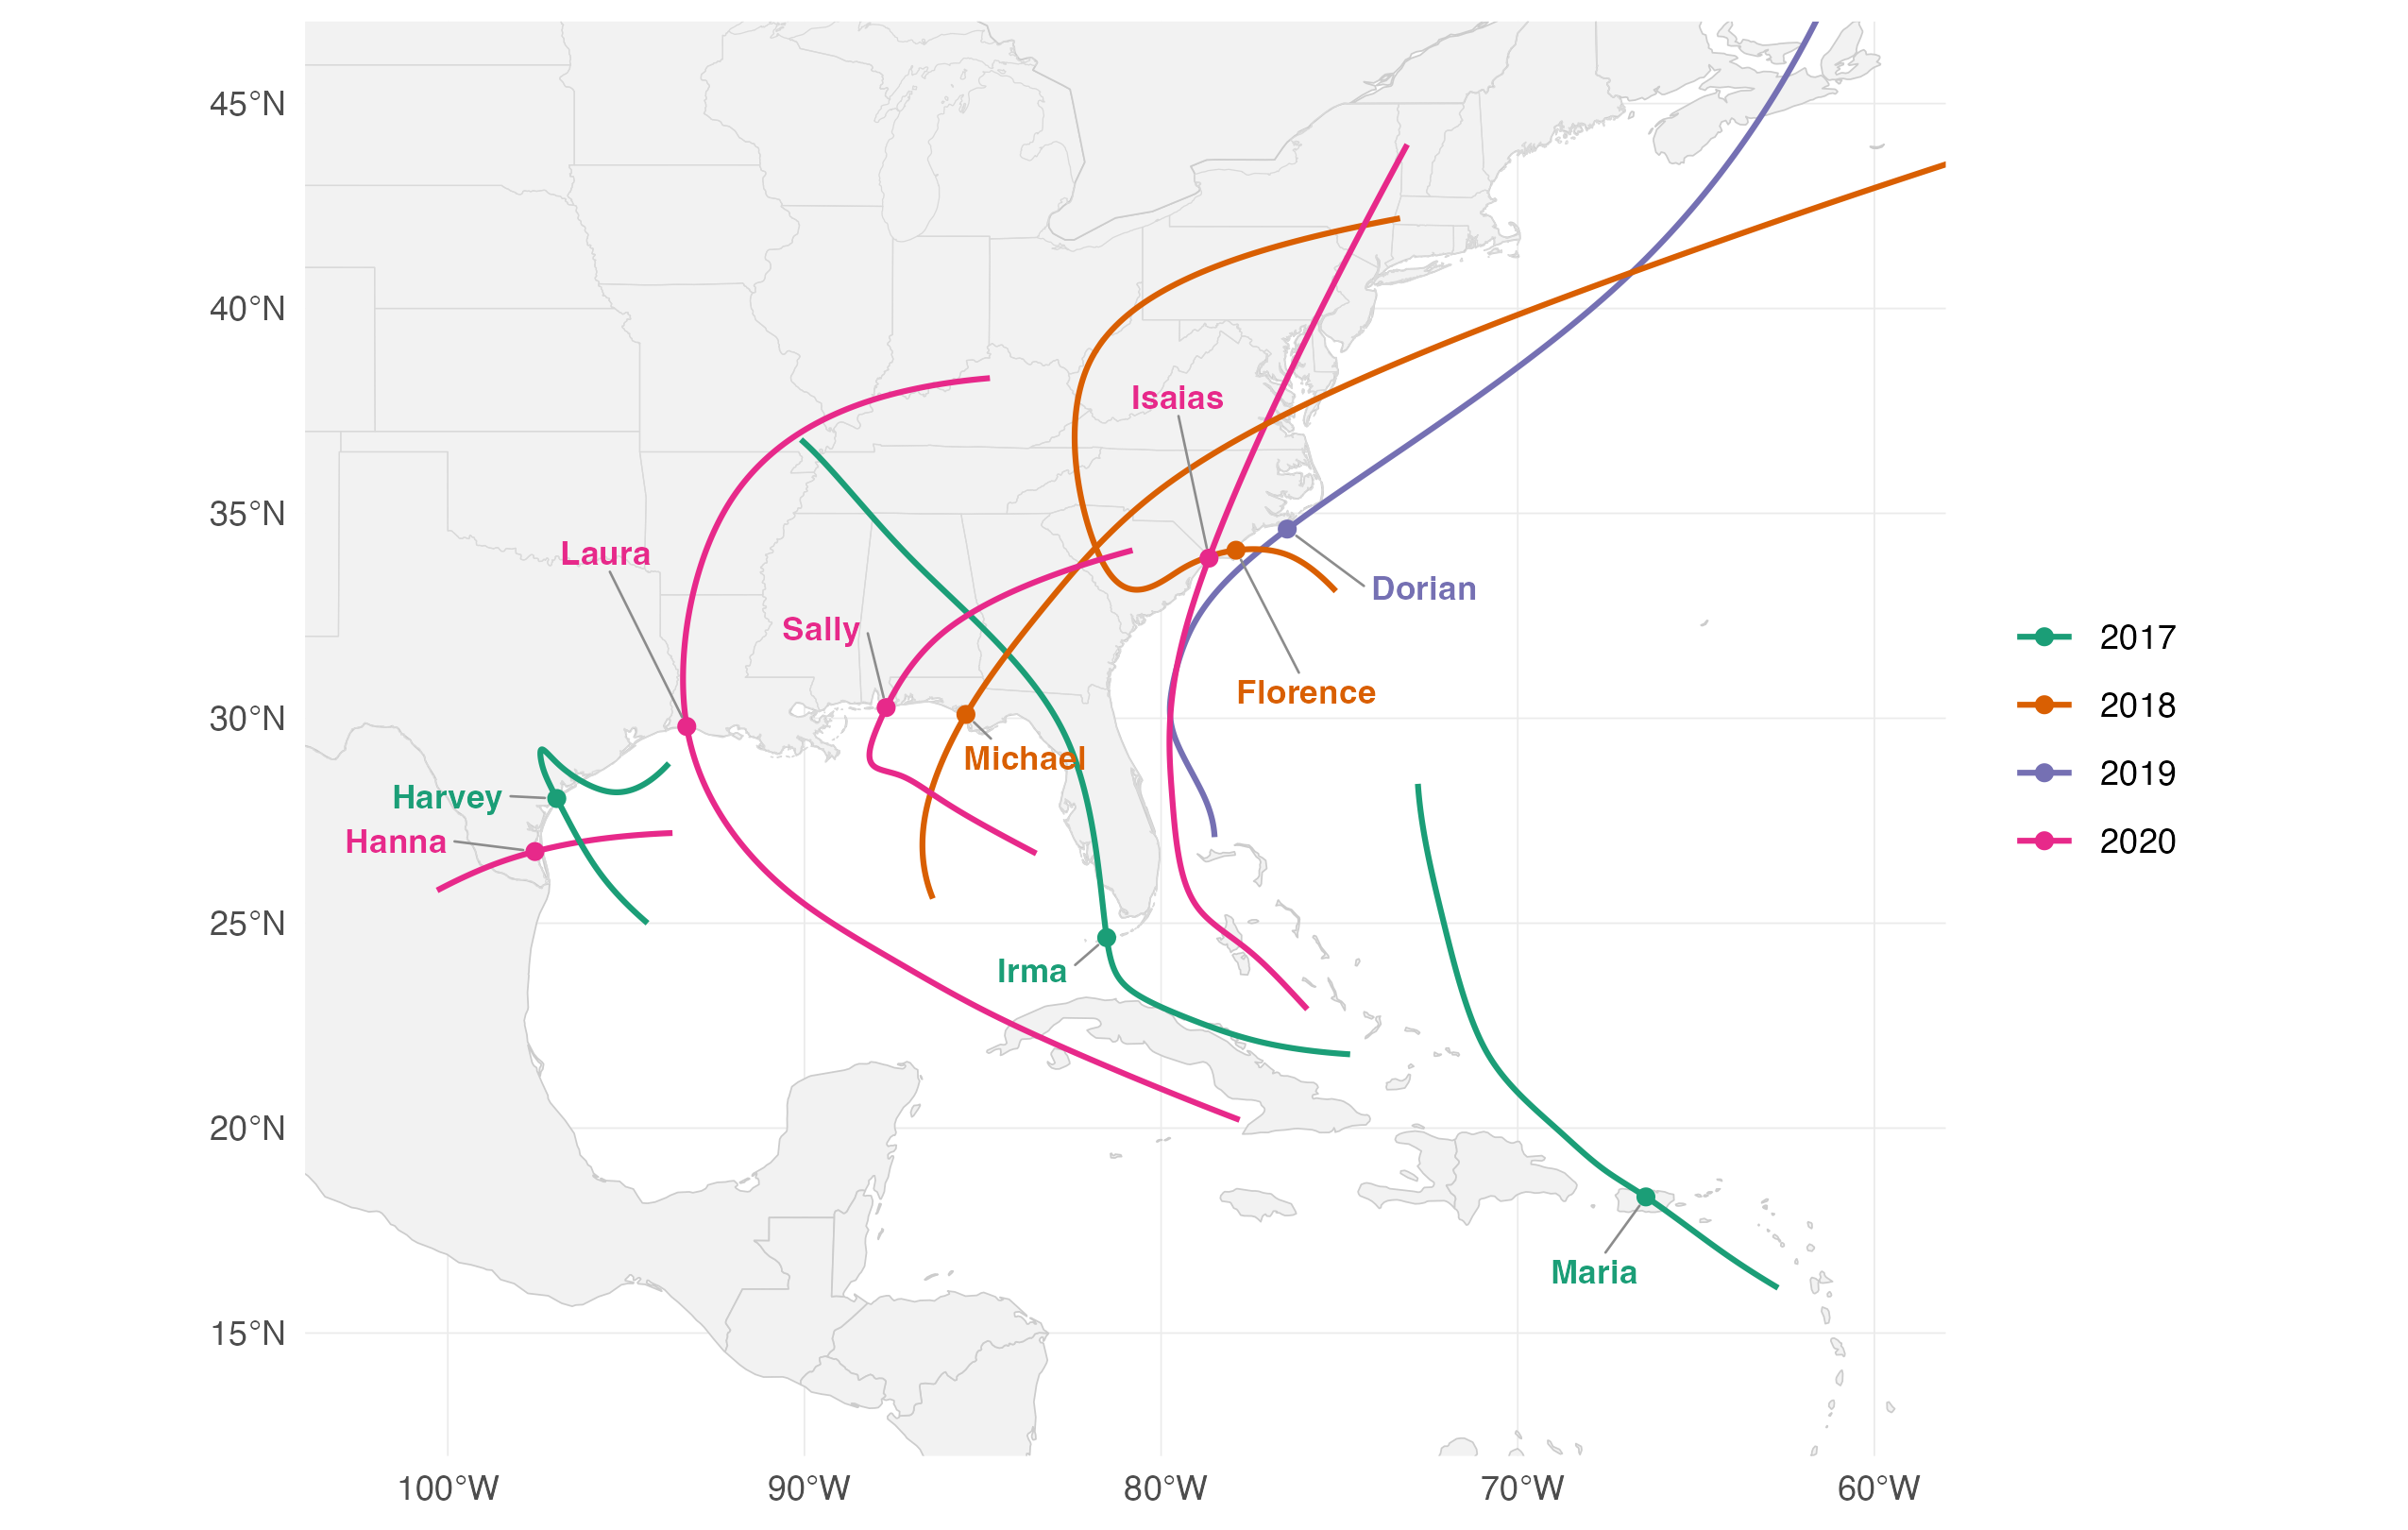
\includegraphics[width=\textwidth]{figures and tables/denial_tracks_map.png}
\caption{Observed tracks of the ten 2017--2020 denial-sample storms, colored by season. Each track is labeled at its US landfall, with Hurricane Maria labeled at its Puerto Rico landfall. \label{fig:denial_tracks}}
\end{figure}

Hurricane Maria enters this denial sample but not the Stage 1 cost panel, a distinction of data availability rather than choice. Stage 1 prices forecast error from realized damages and recovery expenditures, which we observe on a consistent county basis only for the continental United States, so Maria's Puerto Rico landfall lies outside that panel. The denial experiments, by contrast, require no economic data, and Maria's Puerto Rico landfall supplies the high-intensity overland exposures that are among the most informative about the precision gain at hurricane-force winds. We therefore retain Maria wherever the continental cost panel is not needed, namely the Stage 2 precision-gain estimation and the denial-sample valuation in Stage 3.

In this study, augmented observations refer specifically to the dropsonde data that these experiments toggle. The broader institutional definition of AO also includes other aircraft-derived products, such as flight-level wind vectors, central-pressure estimates, and tail radar reflectivity, but the denial design holds these fixed and varies only the dropsondes. We therefore use ``AO'' throughout as shorthand for the dropsonde-assimilated observation set.

This sample is well-suited to our valuation exercise for four reasons: i) the large number of model cycles produced for each storm, ii) the dense dropsonde coverage assimilated into each run, iii) the use of a modern operational-grade forecasting system, and iv) the concentration of high-impact US landfalls within a short window. Following \citet{DitchekEA2023}, we denote the configuration that assimilates all available observations as ``ALL'' and the configuration that \emph{omits} the augmented observations as ``NO.''

The HWRF data-denial experiments deliver deterministic intensity and track forecasts at each lead time, but not the spatial distribution of wind and rainfall over affected counties. To recover that distribution, we apply the same parametric wind and rainfall procedure used to construct $\sigma_{ch}$ in the economic panel \citep{lonfat2007parametric, willoughby2006parametric, knaff2007statistical}, this time seeded by the ALL and NO deterministic forecasts in place of the NHC operational forecast.

For each storm and forecast cycle, we generate 1,000 Monte Carlo synthetic swaths under each assimilation regime, perturbing track and intensity according to the historical NHC forecast-error distribution. Across the ten landfalling hurricanes, this procedure yields roughly 100,000 wind and rainfall swaths, from which county-level ensemble spreads $\sigma_{\text{ALL}}$ and $\sigma_{\text{NO}}$ are computed.

We measure the differential in forecast uncertainty attributable to the reconnaissance network as:
\begin{equation}\label{eq:delta_sigma}
    \Delta \sigma_{AO} \;=\; \sigma_{\text{NO}} - \sigma_{\text{ALL}},
\end{equation}
where $\sigma_{\text{ALL}}$ and $\sigma_{\text{NO}}$ are the county-level ensemble spreads of the parametric swath distributions seeded by the ALL and NO HWRF configurations, respectively. The quantity $\Delta\sigma_{AO}$ isolates the share of forecast uncertainty resolved by augmented observations, which we monetize in Stage 3 by combining it with the loss-function curvature $\hat{\beta}_{2}$ estimated from the economic panel.

%------------------------------------------%
%       Methods
%------------------------------------------%
\section{Estimation and Results} \label{sec:methods}

We operationalize the three-stage framework of Section \ref{sec:model} as follows. Stage 1 estimates the curvature of the loss function from realized damages; Stage 2 estimates the precision gain attributable to AO from the denial experiments; and Stage 3 combines the two into a per-county dollar value. We present each stage's specification alongside its results.

\subsection{Stage 1: The Marginal Cost of Forecast Errors}

We first estimate the curvature of the loss function, $\beta_{2}$, which maps forecast errors to hurricane costs. Estimation relies on the assumption that, conditional on realized storm characteristics and fixed effects, the realization of forecast error is quasi-random.

Let  $c$, $s$, and $h$ index county, state, and hurricane, respectively. The model is then given by:
\begin{align} \label{eq:stage1_reg}
    \text{D}_{csh} \quad
        =&
        \quad \beta^w_2 \left(e^w_{csh}-\mu^w_{csh}\right)^2 + \beta^p_2 \left(e^p_{csh}-\mu^p_{csh}\right)^2 \notag\\
        &+ \sum_{b \in \mathcal{E}^w_i} \gamma^w_b\, \mathbb{1}\{x_{csh} \in b\} + \sum_{b \in \mathcal{E}^p_i} \gamma^p_b\, \mathbb{1}\{p_{csh} \in b\} \notag\\
        & + \gamma_{c} + \eta_{sh} + \varepsilon_{csh}.
\end{align}

Here $\text{D}_{csh}$ is the total ex-post cost, damages plus recovery expenditures. $\left(e^w_{csh}-\mu^w_{csh}\right)^2$ and $\left(e^p_{csh}-\mu^p_{csh}\right)^2$ are the squared demeaned forecast errors in wind speed and precipitation, respectively. $\beta^{w}_{2}$ and $\beta^{p}_{2}$ are the marginal effect of demeaned error on total ex-post cost of wind and precipitation, respectively. We flexibly control for realized wind speed $x_{csh}$ and precipitation $p_{csh}$ with bins, so that identification comes from forecast error conditional on intensity. We include county and state-by-hurricane fixed effects, $\gamma_{c}$ and $\eta_{sh}$, so as to absorb time-invariant county characteristics such as coastal proximity and elevation, and state-level responses to a given storm such as emergency declarations. Standard errors are Conley spatial HAC, allowing for arbitrary serial correlation within a county and spatial correlation across counties within 400 km of its centroid \citep{Conley1999}.

Table \ref{tab:voi-table} reports the coefficient estimates for the squared demeaned wind errors across multiple specifications. Columns (1) through (6) show that the coefficient remains positive and statistically significant across various fixed effect strategies, including county-by-month and county-by-year controls.

\begin{table}

\caption{The Value of a Wind Speed Forecast Improvement. \label{tab:voi-table}}
\centering
\begin{adjustbox}{max width = \textwidth}
\begin{threeparttable}
\begin{tabular}[t]{lccccccc}
\toprule
  & (1) & (2) & (3) & (4) & (5) & (6) & (7)\\
\midrule
\addlinespace[0.5em]
\multicolumn{8}{l}{\textit{Damages + Recovery Expenditures (million \$)}}\\
\midrule \hspace{1em}$\beta_2: (e - \mu)^2$ & 3.74 & 3.73 & 3.25 & 3.26 & 3.75 & 3.65 & \\
\hspace{1em} & (1.32) & (1.32) & (1.06) & (1.00) & (1.34) & (1.19) & \\
\hspace{1em}$\text{Hurricane } \beta_2: (e - \mu)^2$ &  &  &  &  &  &  & 5.03\\
\hspace{1em} &  &  &  &  &  &  & (1.76)\\
\hspace{1em}$\text{Sub-Hurricane } \beta_2: (e - \mu)^2$ &  &  &  &  &  &  & 0.09\\
\hspace{1em} &  &  &  &  &  &  & (0.33)\\
\addlinespace[0.5em]
\multicolumn{8}{l}{\textit{(Damages + Recovery Expenditures) / GDP (\%)}}\\
\midrule \hspace{1em}$\beta_2: (e - \mu)^2$ & 0.20 & 0.21 & 0.18 & 0.18 & 0.18 & 0.18 & \\
\hspace{1em} & (0.06) & (0.06) & (0.05) & (0.05) & (0.05) & (0.05) & \\
\hspace{1em}$\text{Hurricane } \beta_2: (e - \mu)^2$ &  &  &  &  &  &  & 0.28\\
\hspace{1em} &  &  &  &  &  &  & (0.07)\\
\hspace{1em}$\text{Sub-Hurricane } \beta_2: (e - \mu)^2$ &  &  &  &  &  &  & 0.00\\
\hspace{1em} &  &  &  &  &  &  & (0.01)\\
\addlinespace[0.5em]
\multicolumn{8}{l}{\textit{Damages + Recovery Expenditures Per Capita (\$/person)}}\\
\midrule \hspace{1em}$\beta_2: (e - \mu)^2$ & 83.85 & 85.02 & 73.31 & 74.75 & 78.81 & 82.45 & \\
\hspace{1em} & (23.18) & (23.44) & (19.48) & (19.25) & (23.49) & (21.77) & \\
\hspace{1em}$\text{Hurricane } \beta_2: (e - \mu)^2$ &  &  &  &  &  &  & 113.47\\
\hspace{1em} &  &  &  &  &  &  & (28.41)\\
\hspace{1em}$\text{Sub-Hurricane } \beta_2: (e - \mu)^2$ &  &  &  &  &  &  & 2.28\\
\hspace{1em} &  &  &  &  &  &  & (3.28)\\
 &  &  &  &  &  &  \vphantom{1} & \\
Observations & 113,661 & 113,661 & 113,661 & 113,661 & 113,661 & 113,661 & 113,661\\
 &  &  &  &  &  &  & \\
Realized Wind/Precip Bins &  & \checkmark & \checkmark & \checkmark & \checkmark & \checkmark & \checkmark\\
Level Wind/Precip Error &  &  & \checkmark & \checkmark & \checkmark & \checkmark & \checkmark\\
State-Hurricane FE & \checkmark & \checkmark & \checkmark & \checkmark & \checkmark & \checkmark & \checkmark\\
County FE & \checkmark & \checkmark & \checkmark &  &  &  & \checkmark\\
County-Month of Year FE &  &  &  & \checkmark &  & \checkmark & \\
County-Year FE &  &  &  &  & \checkmark & \checkmark & \\
\bottomrule
\end{tabular}
\begin{tablenotes}
\item Standard errors are Conley Spatial HAC with a distance radius of 400 km for spatial correlation
     and arbitrary autocorrelation within counties. $e$ is the county-hurricane-specific forecast
     error, and $\mu$ is the hurricane-intensity bin-specific mean forecast error. Hurricane wind
     speeds are those greater than 33 m/s (74 mph), while Sub-Hurricane wind speeds fall below that
     threshold.
\end{tablenotes}
\end{threeparttable}
\end{adjustbox}
\end{table}


Column (7) presents our preferred specification, which differentiates exposure to hurricane-force ($\geq33$ m/s) and sub-hurricane-force winds. The empirical results show that the cost of forecast error is driven entirely by high-intensity events. For counties experiencing hurricane-force winds, a one-unit increase in the squared demeaned wind speed error increases total costs (damages plus recovery expenditures) by approximately \$5.03 million. In contrast, the effect for sub-hurricane force winds is small and statistically indistinguishable from zero.

This finding aligns with the intuition that protective actions and accurate information are most critical when the physical threat is catastrophic. Consequently, for the remainder of the analysis, we utilize the coefficient $\hat{\beta}^w_{Hurr} = 5.03$ million to value forecast improvements for hurricane-force impacts. We focus on wind throughout: the estimated marginal cost of precipitation forecast error is roughly three orders of magnitude smaller than its wind counterpart and economically negligible (Appendix Table \ref{tab:precip_costs}), so we set precipitation aside and value only wind-speed precision gains. Appendix \ref{app:beta} shows robustness to alternative cost outcomes, the exclusion of individual storms, and using 3-day-ahead forecasts instead of the average of the 1-, 2-, and 3-day-ahead forecasts.

\subsection{Stage 2: AO and Forecast Precision}

In the second stage, we quantify the physical contribution of AO to forecast precision. We utilize the data-denial experiments from \citet{DitchekEA2023} to isolate the reduction in forecast noise attributable to the assimilation of augmented observations.

For each storm $h$ and lead time, we compute the ex-ante error standard deviation (and variance) under two scenarios: the ``No Augmented Observations'' ($\text{NO}$) counterfactual and the ``All Observations'' ($\text{ALL}$) baseline. These are the empirical counterparts of the less- and more-precise forecasts in the model of Section \ref{sec:model}, with $\sigma_{0}=\sigma_{\text{NO}}$ and $\sigma_{1}=\sigma_{\text{ALL}}$. The benefit of the observation network is thus defined as the reduction in the standard deviation of the forecast error:
\begin{equation}
    \Delta \sigma_{h} = \sigma_{\text{NO}, h} - \sigma_{\text{ALL}, h},
\end{equation}
\noindent where $\sigma$ represents the standard deviation of the wind prediction spread. A positive $\Delta \sigma_{h}$ indicates that removing AO increases the dispersion of the forecast signal.

To measure the precision gain we estimate a regression of forecast uncertainty $\sigma$ on the presence of augmented observations, letting the effect vary across the lead-time $\times$ intensity grid. The specification is:
\begin{align}\label{eq:stage2_reg}
   \sigma_{csh}
   &= \text{AO}_{csh}\!\left(\delta + \sum_{\ell\in\{2,3\}}\delta_\ell\,\mathbb{1}\{L_{csh}=\ell\} + \delta_H H_{csh} + \sum_{\ell\in\{2,3\}}\delta_{\ell H}\,\mathbb{1}\{L_{csh}=\ell\}\,H_{csh}\right) \nonumber\\
   &+ \theta \;x_{csh} + \zeta_{L_{csh}H_{csh}} + \alpha_c + \gamma_h + \varepsilon_{csh},
\end{align}
where $\sigma_{csh}$ is the ex-ante wind-speed forecast standard deviation for county $c$ and storm $h$. $\text{AO}_{csh}$ is a dummy equal to 1 when the prediction assimilates augmented observations (the ``ALL'' configuration of \citet{DitchekEA2023}) and 0 otherwise. $L_{csh}$ is the forecast lead time; and $H_{csh}=\mathbb{1}\{x_{csh}\ge 33\text{ m/s}\}$ indicates hurricane-force exposure.

We let the augmented-observation effect vary across the lead-time $\times$ intensity grid. The precision gain in a given cell is the corresponding sum of coefficients. $\theta\,x_{csh}$ controls for realized wind speed, $\zeta_{L_{csh}H_{csh}}$ are lead-by-intensity fixed effects, $\alpha_c$ is a county fixed effect for time-invariant geography, and $\gamma_h$ is a storm fixed effect for storm-specific heterogeneity.

Inference requires special care because the denial experiment is run for entire storms. That is, every county-storm is forecast under both the ALL and NO configurations, so the design is replicated at the storm level. This creates a problem, as the effective number of independent clusters is the number of landfalling hurricanes, which is far too few for asymptotic cluster-robust standard errors to be reliable. To address this issue, we cluster at the storm level and base inference on a wild cluster bootstrap with Webb weights \citep{CameronGelbachMiller2008, Webb2014}.

Table \ref{tab:interaction-grid} reports the results. Columns (1) through (3) pool across all leads and intensities.  The augmented-observation coefficient is positive, small, and statistically indistinguishable from zero, with or without storm fixed effects and the realized-wind control. Realized wind speed is positive and significant, implying that stronger storms are noisier.

\begin{table}

\caption{Precision Gained due to Augmented Observations. \label{tab:interaction-grid}}
\centering
\begin{adjustbox}{max width = \textwidth}
\begin{threeparttable}
\begin{tabular}[t]{lcccccc}
\toprule
  & (1) & (2) & (3) & (4) & (5) & (6)\\
\midrule
$\delta$: Augmented Observations (AO) & 0.015 & 0.015 & 0.015 & -0.055 & -0.055 & -0.055*\\
 & {}[0.645] & {}[0.634] & {}[0.640] & {}[0.104] & {}[0.101] & {}[0.095]\\
$\delta \times$ 2-day lead &  &  &  & 0.146 & 0.145 & 0.145\\
 &  &  &  & {}[0.155] & {}[0.157] & {}[0.165]\\
$\delta \times$ 3-day lead &  &  &  & 0.073 & 0.076 & 0.076\\
 &  &  &  & {}[0.146] & {}[0.136] & {}[0.123]\\
$\delta \times$ Hurricane-force &  &  &  &  & 0.034 & 0.034\\
 &  &  &  &  & {}[0.703] & {}[0.698]\\
$\delta \times$ 2-day $\times$ HF &  &  &  &  & 0.094 & 0.094\\
 &  &  &  &  & {}[0.661] & {}[0.645]\\
$\delta \times$ 3-day $\times$ HF &  &  &  &  & -0.410** & -0.410**\\
 &  &  &  &  & {}[0.035] & {}[0.034]\\
Realized wind speed (m/s) &  &  & 0.256*** & 0.254*** &  & 0.272***\\
 &  &  & {}[0.001] & {}[0.000] &  & {}[0.001]\\
\midrule
Num.Obs. & 115,482 & 115,482 & 115,482 & 115,482 & 115,482 & 115,482\\
R2 & 0.287 & 0.369 & 0.756 & 0.772 & 0.417 & 0.782\\
R2 Adj. & 0.271 & 0.355 & 0.750 & 0.767 & 0.405 & 0.777\\
County FE & \checkmark & \checkmark & \checkmark & \checkmark & \checkmark & \checkmark\\
Storm FE &  & \checkmark & \checkmark & \checkmark & \checkmark & \checkmark\\
Lead-time main effects &  &  &  & \checkmark & \checkmark & \checkmark\\
Intensity main effect &  &  &  &  & \checkmark & \checkmark\\
\bottomrule
\end{tabular}
\begin{tablenotes}
\item * p $<$ 0.1, ** p $<$ 0.05, *** p $<$ 0.01 HF denotes hurricane-force realizations, wind $\geq$ 33 m/s; the reference category is 1-day-lead, sub-hurricane-force forecasts. ``Lead-time main effects'' are the 2- and 3-day lead indicators and ``Intensity main effect'' the hurricane-force indicator. Square brackets report wild cluster bootstrap $p$-values with Webb weights, on which the stars are based.
\end{tablenotes}
\end{threeparttable}
\end{adjustbox}
\end{table}


Column (4) lets the effect vary by lead time, and columns (5) and (6) add its interaction with intensity to recover the full lead $\times$ intensity grid, without and with the realized-wind control. A clear pattern arises: augmented observations reduce ex-ante uncertainty, in average, by 0.055 m/s after controlling for lead time. The augmented-observation $\times$ 3-day $\times$ hurricane-force term reduces the forecast spread by a further 0.41 m/s, an estimate left essentially unchanged by the realized-wind control. We interpret this as evidence that the meaningful precision gain is concentrated in the 3-day hurricane-force prediction, where summing $\delta$ with its 3-day, hurricane-force, and 3-day $\times$ hurricane-force components implies a reduction of 0.356 m/s.

While 0.356 m/s is modest in absolute terms, it represents a meaningful share of the forecast noise. Compared against all 3-day forecasts in the panel (pooling all storm intensities, mean $\bar{\sigma}_{\text{ALL}} \approx 2.13$ m/s), $\delta$ represents about a 17\% reduction due to AO. When the comparison is restricted to the hurricane-force subsample that drives the valuation in Stage 3 ($\bar{\sigma}_{\text{ALL}} \approx 10.13$ m/s with AO assimilated), $\delta$ represents a reduction of about 3.5\%. We will carry the point estimate $\hat{\delta}_{3,\text{HF}} = 0.356$ m/s into the valuation below. Appendix \ref{app:delta} documents its robustness to lead time, intensity, and the exclusion of individual storms.

\subsection{Stage 3: Projecting Economic Gains}

In the final stage, we monetize the precision gains identified in Stage 2 by applying the valuation identity in Equation \eqref{eq:voi_finite}. Combining the Stage 1 estimate of the loss-function curvature for wind, $\hat{\beta}^w_{Hurr}$, with the Stage 2 estimate of the precision differential, $\hat{\delta}$, the storm- and county-specific social value of AO is:
\begin{equation} \label{eq:value_calc}
     V^{AO}_{csh} \;=\; \hat{\beta}^w_{Hurr} \,\left[(\sigma_{\text{ALL},h} + \hat{\delta}_{3,\text{HF}})^{2} - \sigma_{\text{ALL},h}^{2}\right].
\end{equation}

Following the linear approximation established in Section \ref{sec:model}, this calculation simplifies to $V^{AO}_{csh} \approx 2\,\hat{\beta}^w_{Hurr}\times\sigma_{\text{ALL},h}\times\hat{\delta}_{3,\text{HF}}$. This operational form explicitly highlights how the final monetary benefits scale with a storm's baseline uncertainty under the active observation regime $\sigma_{\text{ALL},h}$.

We therefore monetize the precision gain in the 3-day hurricane-force cell that Stage 2 identifies. Evaluating the per-county value $\hat{\beta}^w_2\,[(\bar{\sigma}_{\text{ALL}}+\hat{\delta})^2 - \bar{\sigma}_{\text{ALL}}^2]$ across the full lead-time $\times$ intensity grid confirms that the value concentrates in this cell: for sub-hurricane exposures it is negligible, because the marginal cost of forecast error is statistically indistinguishable from zero below hurricane force (Table \ref{tab:voi-table}).

Putting these pieces together, we project the economic value of the observational improvements. AO reduce the forecast standard deviation by approximately $\hat{\delta} = 0.356$ m/s at the 3-day lead time. With an average baseline forecast uncertainty $\bar{\sigma}_{\text{ALL}}$ of approximately 10.13 m/s for the hurricanes in the sample, the 0.356 m/s physical improvement translates to a reduction in variance of roughly 7.3 (m/s)$^2$.\footnote{Recall that the value of a forecast improvement is proportional to the reduction in error variance: $\sigma_{\text{NO}}^{2} - \sigma_{\text{ALL}}^{2} \approx 2\bar{\sigma}_{\text{ALL}}\hat{\delta}$.} Scaling this variance reduction by the marginal cost parameter ($\hat{\beta}^w_{Hurr} = 5.03$ million) yields an estimated benefit of AO of approximately \$36.9 million per county per storm, for counties predicted to be exposed to hurricane-force winds.

We can now directly derive the total value of augmented observations. We note that for the storms with aircraft reconnaissance between 2017 and 2020, 137 counties were predicted to experience hurricane-force wind speeds. This implies that the total retrospective social value of the AO in this time period is approximately \$5.05 billion.

\subsection{Cost-Benefit Analysis}

Here, we use published official benchmarks of the social return on NOAA's hurricane research aircraft platform. The main source is the 2016 Analysis of Alternatives (AoA) commissioned by NOAA's Office of Marine and Aviation Operations \citep{ANSER2016ExternalBenefits}. That study quantified four direct benefit channels. Namely, the reduction of needless evacuations (\$139 million), commercial air traffic disruption (\$134 million), negligible commercial maritime traffic disruption (under \$1 million), and benefits to atmospheric chemistry research (\$228 million). Their calculations indicate a total NPV of approximately \$501 million (base-year \$2024, $r = 7\%$) over the 25-year operating life of an observation platform. The life-cycle cost of the least-cost alternative considered (two modified Lockheed C-130J aircraft) was \$680 million NPV over the same horizon, yielding a base-case benefit-to-cost ratio of approximately 0.75:1. 

Our framework expands on this baseline and it provides the social value associated with the ex ante variance reduction in the wind-speed forecast as captured by damages and public assistance grants. On the 2017--2020 retrospective denial sample, this single channel yields a social value of approximately \$5.05 billion or roughly 10 times the entire 2030--2055 NPV that the AoA estimated. Annualized over the four years of data-denial experiments, the implied benefit rate is approximately \$1.26 billion per year. 

The implications for the ongoing recapitalization are stark. The 2022 NOAA Aircraft Recapitalization Plan \citep{NOAA2022AircraftPlan} initiated the procurement of four C-130J aircraft to replace the aging WP-3D fleet, with a total acquisition cost subsequently estimated at approximately \$1.4 billion \citep{GAO2025HurricaneHunter}, of which roughly \$678 million remained to be funded as of January 2025. The retrospective social value from a single four-year window of operations under our framework exceeds the entire undiscounted acquisition cost of the replacement fleet by more than threefold, and exceeds the remaining unfunded balance by more than seven times.

Importantly, our headline figure isolates the \emph{dropsonde-attributable} channel of aircraft reconnaissance. Because other onboard sensors, such as flight-level wind vectors, central-pressure estimates, and tail radar reflectivity, are held constant across both the ALL and NO configurations, our valuation should be interpreted as a conservative lower bound on the aggregate social value delivered by the NOAA aircraft infrastructure.


Finally, our \$5.05 billion figure reflects only the seven storms in the 2017--2020 denial archive. Augmented observations have been flown for essentially every hurricane threatening the continental United States since the HWRF model became operational in 2007 \citep{AlakaJr2024}. Applying the same per-county valuation to every hurricane-force, 3-day-lead county-storm in the continental forecast panel over 2007--2024, and holding the precision gain fixed at its denial-sample estimate (which we believe is a conservative assumption as the quality of the forecast has gone up over time) suggests cumulative benefits on the order of \$6.2 billion, or roughly \$340 million per year (Appendix \ref{app:per-storm}).

%------------------------------------------%
%       Discussion and Conclusion 
%------------------------------------------%
\section{Discussion} \label{sec:discussion}

In this paper we estimate the social value of augmented aircraft observations in hurricane forecasting. We find that the social cost of forecast error is concentrated in the most intense storms, and that augmented observations meaningfully reduce the forecast standard deviation three days before landfall for the most intense storms as well. Monetizing this precision gain through an estimated cost function yields roughly \$36.9 million in social value per county predicted to experience hurricane-force winds. These results suggest that in-situ reconnaissance delivers value precisely where forecast errors are most costly, in the severe and hard-to-predict storms that drive the bulk of hurricane losses.

We also provide an aggregate estimate of the return of investment to this reconnaissance program. Across the 2017--2020 sample that lets us establish the contribution of these observations to forecast precision, augmented observations generated approximately \$5.05 billion in social value, or more than 3.5 times the \$1.4 billion acquisition cost of NOAA's planned fleet recapitalization. A back-of-the-envelope extrapolation to every continental hurricane observed since the HWRF model became operational in 2007 places the cumulative value on the order of \$6.2 billion.

These magnitudes speak directly to the policy environment that motivates this paper. Recent budget proposals would have sharply reduced funding across the federal forecasting enterprise, from NOAA's research offices \citep{CRS2026NOAABudget} to the National Science Foundation programs that sustain the National Center for Atmospheric Research \citep{NSF2025BudgetRequest, Science2025NCAR}, while reduction-in-force directives reached staffing at the National Weather Service and the National Hurricane Center \citep{EO14210Workforce2025}. Although much of this funding was subsequently restored \citep{witze2026world}, the episode illustrates how exposed observing and forecasting infrastructure is to short-run fiscal pressure. Our estimates supply the term that such decisions most often lack: the social value generated by a single observing channel runs into the billions and exceeds the cost of the aircraft that produce it by a wide margin, so scaling back reconnaissance, or the assimilation systems that turn it into forecasts, would forgo returns that are large, quantifiable, and concentrated in the high-intensity storms where public protection matters most.

More broadly, our approach offers a way to value public investment in information itself. Forecasting infrastructure is rarely evaluated on the same empirical footing as physical protection such as levees or sea walls \citep{fried2022seawalls}, because its benefits are diffuse and realized only in expectation. Pricing the precision that observations deliver converts that diffuse benefit into a figure that can be weighed against an appropriation. As scrutiny of public science budgets intensifies, which is in itself desirable and needed, valuations of this kind are likely to become central to deciding what societies choose to observe, fund, and how well.

The same logic extends well beyond hurricane reconnaissance. NOAA is making large contemporaneous investments across the observing and forecasting enterprise whose social returns remain similarly unpriced. On the observing side, the Space Weather Follow On-Lagrange 1 observatory (SWFO-L1) now tracks solar activity upstream of Earth \citep{NOAA_SWFOL1_2025}, and the Sentinel-6B altimeter extends a multi-decade record of sea-surface height that feeds storm-surge and coastal prediction \citep{NOAA_Sentinel6B_2025}. On the computing and modeling side, the Rhea high-performance system adds dedicated capacity for machine-learning-based prediction \citep{NOAA_Rhea_2024}, and Project EAGLE has begun operationalizing AI-based global forecast models \citep{NOAA_ProjectEAGLE_2025}. Each of these is justified today largely through the assumption-based accounting our framework is designed to replace. Wherever a system's physical contribution to forecast precision can be isolated, the same two-stage approach proposed here can convert it into a dollar-denominated social return, putting funding decisions across very different infrastructure on a common empirical footing.

We conclude with several limitations that we leave for future work. First, our valuation prices wind-speed precision alone. Wind is the leading driver of hurricane damage \citep{HilderbrandXie2025}, but inland flooding and storm surge are consequential as well, and surge forecasting in particular remains less mature than track and intensity prediction. Augmented observations plausibly sharpen these forecasts too, so valuing their precision along these additional dimensions would only raise the estimated return.

Second, we price the contraction of forecast uncertainty and abstract from the channels through which that information ultimately reduces losses. Our framework is agnostic to the specific protective actions that households and agencies take in response to a forecast, and it does not separately value the longer-run social-insurance costs \citep{deryugina2017fiscal} or the mortality impacts that improved forecasts may mitigate. Incorporating these margins, like the multi-hazard channels above, would push the valuation upward rather than downward.

Third, our valuation counts only damages within the United States, even though augmented observations improve the forecasts used across the entire Atlantic basin. The dropsondes assimilated for a given storm sharpen its track and intensity guidance regardless of where it ultimately makes landfall, so the same reconnaissance we price through US damages also helps the Caribbean islands, Mexico, and Central American. nations  that lie in the path of many Atlantic hurricanes prepare for them. The estimates here omit these benefits abroad and therefore understate the overall program's full social return at a global scale.

Fourth, our analysis relies on data-denial experiments covering storms from the 2017 to 2020 seasons. While this sample successfully establishes our framework, institutionalizing these experiments across all operational forecasts would transform the ability to value scientific infrastructure. If running counterfactual forecasts becomes a routine practice, this valuation approach scales effortlessly. It can extend naturally beyond aircraft reconnaissance to price the satellite, radiosonde, and ocean-observing networks that initialize forecasts worldwide. Ultimately, making these evaluations standard practice would provide policymakers with a continuous, empirical foundation for funding the global meteorological enterprise.

Fifth, we hold the 3-day forecast lead fixed throughout. This is the horizon that governs pre-landfall protective decisions, but it leaves unmeasured the value of earlier and more frequent reconnaissance, which recent advances in forecasting may amplify, and the gains from extending precise guidance further ahead of landfall. As coastal exposure grows and tropical-cyclone behavior becomes harder to predict, quantifying the value of the observations that initialize hurricane forecasts is likely to remain a first-order question for both meteorology and economics.

%------------------------------------------%
%                References
%------------------------------------------%
\FloatBarrier
\newpage
\begin{singlespace}
\bibliographystyle{references/econ}
\bibliography{references/references}{}
\end{singlespace}
%------------------------------------------%
%                Appendix
%------------------------------------------%
\FloatBarrier
\clearpage
\appendix

% --- Appendix title page ---
\thispagestyle{empty}
\begin{center}
\vspace*{\fill}
{\LARGE\bfseries APPENDIX \\ Hurricane Hunters and Economic Value of Hurricane Forecasting Augmented Observations\par}
\vspace{0.7cm}
{\Large by Diego Cardoso, Mark DeMaria, Brian McNoldy, Renato Molina, David Nolan, and Ivan Rudik\par}
\vspace*{\fill}
\end{center}
\clearpage

% Reset figure/table #'s
\setcounter{table}{0}
% Number tables by appendix section: A1, A2, ... in Appendix A; B1, ... in Appendix B; etc.
\counterwithin{table}{section}
\renewcommand{\thetable}{\thesection\arabic{table}}
% Place appendix tables exactly where input (after the prose), not floated to page tops
\floatplacement{table}{H}

\begin{appendices}

% ============================================================================
% Appendix A — beta robustness on the VOI panel
% ============================================================================
\section{Robustness of the Marginal Cost Parameter} \label{app:beta}

Here we show that the Stage 1 marginal cost of forecast error $\hat{\beta}^w_{Hurr}$ is robust across a range of empirical choices. We assess sensitivity to the cost outcome, to the exclusion of individual storms, and to the forecast lead, and we document why we value wind-speed precision rather than precipitation. Taken together, the estimate is stable and the headline valuation is not an artifact of any single choice.

We first vary the cost outcome. Table \ref{tab:cost_outcomes} re-estimates the Stage 1 marginal cost $\hat{\beta}^w_{Hurr}$ on total cost, cost per county GDP, and cost per capita; the coefficient is positive, significant, and of the same order of magnitude across all three, so the estimate is not an artifact of weighting the panel by population or economy size.

Table \ref{tab:implied_value} carries each of these coefficients through the Stage 3 valuation. The resulting aggregate social values are of comparable magnitude, so the headline retrospective figure does not depend on how the cost outcome is normalized.

We next drop one storm at a time. Table \ref{tab:cost_jackknife} brackets the \$5.03 million baseline between \$3.50 million (Katrina removed) and \$6.80 million (Michael removed), so no single storm drives the parameter.

Because the social value concentrates at the 3-day lead, we re-estimate the marginal cost on the 3-day-ahead forecast error alone rather than the 1--3 day average. Table \ref{tab:cost_3day} returns a hurricane-force coefficient of \$3.80 million, statistically indistinguishable from the pooled-lead baseline, while the sub-hurricane effect remains near zero.

Finally, we report the full specification with the precipitation forecast-error coefficient that the main table omits. Table \ref{tab:precip_costs} shows it is negligible and statistically indistinguishable from zero, which is why we value wind-speed precision and set precipitation aside.

\clearpage

\begin{table}

\caption{Outcome robustness for the preferred specification (2005--2024 panel). \label{tab:cost_outcomes}}
\centering
\begin{adjustbox}{max width = \textwidth}
\begin{threeparttable}
\begin{tabular}[t]{lccc}
\toprule
  & Total cost (million \$) & Cost / county GDP (\%) & Cost per capita (\$/person)\\
\midrule
$\text{Hurricane } \beta_2: (e - \mu)^2$ & 5.03*** & 0.28*** & 113.47***\\
 & (1.76) & (0.07) & (28.41)\\
$\text{Sub-Hurricane } \beta_2: (e - \mu)^2$ & 0.09 & 0.00 & 2.28\\
 & (0.33) & (0.01) & (3.28)\\
\bottomrule
\end{tabular}
\begin{tablenotes}
\item * p $<$ 0.1, ** p $<$ 0.05, *** p $<$ 0.01. Preferred specification (Table \ref{tab:voi-table}), with Conley spatial HAC standard errors with a 400 km cutoff.
\end{tablenotes}
\end{threeparttable}
\end{adjustbox}
\end{table}

\begin{table}

\caption{Implied retrospective social value of augmented observations under three notions of value. \label{tab:implied_value}}
\centering
\begin{adjustbox}{max width = \textwidth}
\begin{threeparttable}
\begin{tabular}[t]{lrrr}
\toprule
Outcome variable & $\hat{\beta}^w_{Hurr}$ & Mean per-county value (\$M) & Aggregate value 2017--2020 (\$B)\\
\midrule
Total cost (\$M) & 3.799 & 27.85 & 3.82\\
Cost / county GDP (\%) & 0.178 & 60.46 & 3.75\\
Cost per capita (\$) & 76.440 & 51.62 & 3.20\\
\bottomrule
\end{tabular}
\begin{tablenotes}
\small
\item The total-cost aggregate sums over all 137 hurricane-force county-storms including Maria. The cost/GDP and cost-per-capita columns sum over the 62 continental county-storms with observed GDP and population.
\end{tablenotes}
\end{threeparttable}
\end{adjustbox}
\end{table}


\begin{table}

\caption{One-storm-out jackknife of the marginal cost of forecast error. \label{tab:cost_jackknife}}
\centering
\begin{adjustbox}{max width = \textwidth}
\begin{threeparttable}
\begin{tabular}[t]{lrrr}
\toprule
Dropped & Obs. & $\beta_2$: Hurricane & $\beta_2$: Sub-Hurr.\\
\midrule
(none) & 113,661 & 5.031 (1.760) & 0.095 (0.330)\\
Katrina & 110,588 & 3.504 (0.870) & 0.036 (0.306)\\
Harvey & 110,588 & 4.841 (1.853) & -0.193 (0.227)\\
Sandy & 110,588 & 4.978 (1.742) & 0.072 (0.328)\\
Ian & 110,588 & 4.772 (1.829) & 0.237 (0.334)\\
Ida & 110,588 & 5.320 (2.049) & 0.103 (0.343)\\
Michael & 110,588 & 6.795 (2.153) & 0.192 (0.330)\\
Laura & 110,588 & 5.188 (2.078) & 0.119 (0.342)\\
Irma & 110,588 & 5.045 (1.770) & 0.095 (0.331)\\
Wilma & 110,588 & 4.707 (1.691) & 0.044 (0.328)\\
Rita & 110,588 & 4.958 (1.793) & 0.056 (0.334)\\
Helene & 110,596 & 5.034 (1.807) & -0.016 (0.425)\\
\bottomrule
\end{tabular}
\begin{tablenotes}
\small
\item Each row reports preferred-specification estimates after dropping the indicated storm from the panel. Conley Spatial HAC standard errors (400 km cutoff) in parentheses. The baseline row drops no storm.
\end{tablenotes}
\end{threeparttable}
\end{adjustbox}
\end{table}

\begin{table}

\caption{Marginal cost of forecast error using 3-day-ahead forecasts only. \label{tab:cost_3day}}
\centering
\setlength{\tabcolsep}{26pt}
\begin{adjustbox}{max width = \textwidth}
\begin{threeparttable}
\begin{tabular}[t]{lcc}
\toprule
  & Baseline & 3-day only\\
\midrule
$\text{Hurricane } \beta^{w}_{2}: (e-\mu)^2$ & 5.03*** & 3.80**\\
 & (1.76) & (1.85)\\
$\text{Sub-Hurricane } \beta^{w}_{2}: (e-\mu)^2$ & 0.09 & 0.06\\
 & (0.33) & (0.12)\\
 &  & \\
Observations & 113,661 & 75,512\\
Realized Wind/Precip Bins & \checkmark & \checkmark\\
State-Hurricane FE & \checkmark & \checkmark\\
County FE & \checkmark & \checkmark\\
\bottomrule
\end{tabular}
\begin{tablenotes}
\item * p $<$ 0.1, ** p $<$ 0.05, *** p $<$ 0.01 Preferred specification (Table \ref{tab:voi-table}) on total cost. Column (1) uses the 1--3 day average forecast error, column (2) the 3-day-ahead error only. Conley spatial HAC standard errors with a 400 km cutoff.
\end{tablenotes}
\end{threeparttable}
\end{adjustbox}
\end{table}

\begin{table}

\caption{Wind and Precipitation Forecast-Error Costs. \label{tab:precip_costs}}
\centering
\begin{adjustbox}{max width = \textwidth}
\begin{threeparttable}
\begin{tabular}[t]{lccccccc}
\toprule
  & (1) & (2) & (3) & (4) & (5) & (6) & (7)\\
\midrule
Wind, $\beta^w_2: (e^w - \mu^w)^2$ & 3.741*** & 3.731*** & 3.248*** & 3.261*** & 3.748*** & 3.646*** & \\
 & (1.316) & (1.323) & (1.059) & (1.001) & (1.338) & (1.195) & \\
Wind, Hurricane $\beta^w_2$ &  &  &  &  &  &  & 5.031***\\
 &  &  &  &  &  &  & (1.760)\\
Wind, Sub-Hurricane $\beta^w_2$ &  &  &  &  &  &  & 0.095\\
 &  &  &  &  &  &  & (0.330)\\
Precipitation, $\beta^p_2: (e^p - \mu^p)^2$ & 0.003 & 0.001 & 0.003 & 0.004 & 0.003 & 0.006* & 0.003\\
 & (0.005) & (0.005) & (0.003) & (0.003) & (0.003) & (0.003) & (0.003)\\
 &  &  &  &  &  &  & \\
Observations & 113,661 & 113,661 & 113,661 & 113,661 & 113,661 & 113,661 & 113,661\\
 &  &  &  &  &  &  & \\
Realized Wind/Precip Bins &  & \checkmark & \checkmark & \checkmark & \checkmark & \checkmark & \checkmark\\
Level Wind/Precip Error &  &  & \checkmark & \checkmark & \checkmark & \checkmark & \checkmark\\
State-Hurricane FE & \checkmark & \checkmark & \checkmark & \checkmark & \checkmark & \checkmark & \checkmark\\
County FE & \checkmark & \checkmark & \checkmark &  &  &  & \checkmark\\
County-Month of Year FE &  &  &  & \checkmark &  & \checkmark & \\
County-Year FE &  &  &  &  & \checkmark & \checkmark & \\
\bottomrule
\end{tabular}
\begin{tablenotes}
\item * p $<$ 0.1, ** p $<$ 0.05, *** p $<$ 0.01 Full coefficient table for the Stage 1 value-of-information regressions, reporting both the
     wind ($\beta^w_2$) and precipitation ($\beta^p_2$) squared demeaned forecast-error
     coefficients; the main table omits precipitation. $e$ is the county-hurricane-specific forecast
     error and $\mu$ the hurricane-intensity bin-specific mean forecast error. Hurricane wind
     speeds exceed 33 m/s (74 mph); Sub-Hurricane wind speeds fall below that threshold. Standard
     errors are Conley Spatial HAC with a 400 km distance radius.
\end{tablenotes}
\end{threeparttable}
\end{adjustbox}
\end{table}


\clearpage


% ============================================================================
% Appendix B — delta robustness on the denial panel
% ============================================================================
\section{Robustness of the Precision Gain} \label{app:delta}

Here we show that the Stage 2 precision gain $\delta$ is robust. We first report the full lead $\times$ intensity interaction that identifies it, and then confirm that the result survives dropping any single storm from the denial sample.

Table \ref{tab:precision_full} reports the full lead $\times$ intensity interaction behind the Stage 2 precision gain. The gain $\delta$ rises from a negligible 0.021 m/s at the 1-day lead to 0.356 m/s at 3 days, and the identified effect is the augmented-observation $\times$ 3-day $\times$ hurricane-force triple ($-0.410$ m/s), the only term significant under the wild cluster bootstrap.

We then drop one storm at a time and re-estimate that triple. Table \ref{tab:precision_jackknife_maria} shows the coefficient stays between $-0.347$ and $-0.432$ m/s and significant in every case except the removal of Hurricane Maria. Here we note that Maria contributes the bulk of the hurricane-force / 3-day-lead observations, yet dropping it leaves the estimate essentially unchanged at $-0.397$ m/s ($p = 0.10$).

\clearpage


% Tables in the order they are discussed above (para 1: full interaction; para 2: jackknife of the triple)
\begin{table}

\caption{Full coefficient estimates for the augmented-observations precision regression. \label{tab:precision_full}}
\centering
\begin{adjustbox}{max width = \textwidth}
\begin{threeparttable}
\begin{tabular}[t]{lcccccc}
\toprule
  & (1) & (2) & (3) & (4) & (5) & (6)\\
\midrule
$\delta$: Augmented Observations (AO) & 0.015 & 0.015 & 0.015 & -0.055* & -0.055* & -0.055*\\
 & {}[0.634] & {}[0.634] & {}[0.635] & {}[0.095] & {}[0.092] & {}[0.091]\\
2-day lead &  &  &  & 0.296*** & 0.298*** & 0.297***\\
 &  &  &  & {}[0.001] & {}[0.000] & {}[0.000]\\
3-day lead &  &  &  & 0.665*** & 0.658*** & 0.657***\\
 &  &  &  & {}[0.004] & {}[0.005] & {}[0.005]\\
Hurricane-force (HF) &  &  &  &  & 5.653*** & 1.913***\\
 &  &  &  &  & {}[0.001] & {}[0.009]\\
$\delta \times$ 2-day lead &  &  &  & 0.146 & 0.145 & 0.145\\
 &  &  &  & {}[0.139] & {}[0.152] & {}[0.155]\\
$\delta \times$ 3-day lead &  &  &  & 0.073 & 0.076 & 0.076\\
 &  &  &  & {}[0.155] & {}[0.139] & {}[0.136]\\
$\delta \times$ Hurricane-force &  &  &  &  & 0.034 & 0.034\\
 &  &  &  &  & {}[0.710] & {}[0.697]\\
2-day lead $\times$ HF &  &  &  &  & -0.211 & -0.185\\
 &  &  &  &  & {}[0.896] & {}[0.917]\\
3-day lead $\times$ HF &  &  &  &  & 0.851* & 0.973*\\
 &  &  &  &  & {}[0.051] & {}[0.060]\\
$\delta \times$ 2-day $\times$ HF &  &  &  &  & 0.094 & 0.094\\
 &  &  &  &  & {}[0.659] & {}[0.638]\\
$\delta \times$ 3-day $\times$ HF &  &  &  &  & -0.410** & -0.410**\\
 &  &  &  &  & {}[0.030] & {}[0.029]\\
\midrule
Num.Obs. & 115,482 & 115,482 & 115,482 & 115,482 & 115,482 & 115,482\\
County FE & \checkmark & \checkmark & \checkmark & \checkmark & \checkmark & \checkmark\\
Storm FE &  & \checkmark & \checkmark & \checkmark & \checkmark & \checkmark\\
Forecast-wind bins &  &  & \checkmark & \checkmark &  & \checkmark\\
\bottomrule
\end{tabular}
\begin{tablenotes}
\item * p $<$ 0.1, ** p $<$ 0.05, *** p $<$ 0.01 Full coefficient vector of the precision regression, of which the main text reports only the augmented-observation terms. HF denotes hurricane-force realizations ($\geq$ 33 m/s), with 1-day-lead sub-hurricane forecasts as the reference. Square brackets report wild cluster bootstrap $p$-values with Webb weights, on which the stars are based.
\end{tablenotes}
\end{threeparttable}
\end{adjustbox}
\end{table}

\begin{table}

\caption{One-storm-out jackknife of the augmented-observation $\times$ 3-day $\times$ hurricane-force interaction. \label{tab:precision_jackknife_maria}}
\centering
\begin{adjustbox}{max width = \textwidth}
\begin{threeparttable}
\begin{tabular}[t]{lrrr}
\toprule
Dropped & Obs. & $\delta_{3,\text{HF}}$ (m/s) & Bootstrap $p$\\
\midrule
(None) & 115,482 & -0.410** & 0.033\\
Dorian & 101,106 & -0.426** & 0.023\\
Florence & 101,106 & -0.425** & 0.027\\
Hanna & 110,690 & -0.432** & 0.016\\
Harvey & 105,898 & -0.397** & 0.037\\
Irma & 101,106 & -0.347* & 0.059\\
Isaias & 101,106 & -0.426** & 0.030\\
Laura & 101,106 & -0.426* & 0.051\\
Maria & 115,008 & -0.397 & 0.104\\
Michael & 101,106 & -0.416* & 0.088\\
Sally & 101,106 & -0.398** & 0.034\\
\bottomrule
\end{tabular}
\begin{tablenotes}
\small
\item Triple-interaction coefficient $\delta_{3,\text{HF}}$ from the full interaction (Table \ref{tab:precision_full}), re-estimated after dropping each storm. Significance from a restricted wild cluster bootstrap with Webb weights (B = 1999, clustered on storm).
\end{tablenotes}
\end{threeparttable}
\end{adjustbox}
\end{table}


\clearpage

% ============================================================================
% Appendix C — per-storm decomposition of the retrospective valuation
% ============================================================================
\section{Per-Storm Decomposition of the Retrospective Social Value} \label{app:per-storm}

Here we look more closely at where the headline retrospective value comes from. We first decompose it across the individual storms in the denial sample, and then set it against the cost of the replacement-platform alternatives the program would fund.

Table \ref{tab:per_storm} decomposes the \$5.05 billion retrospective value by storm, pricing each at its own baseline forecast uncertainty so that storm $h$ contributes its hurricane-force / 3-day-lead county count times $\hat{\beta}^w_{Hurr}\,[(\bar{\sigma}_{\text{ALL},h}+\hat{\delta})^2 - \bar{\sigma}_{\text{ALL},h}^2]$. The total is dominated by Hurricane Maria (\$3.0 billion, 60\%), reflecting both its county count and its unusually high baseline forecast uncertainty.

Table \ref{tab:platform_comparison} sets our estimated benefits against the cost of replacing the fleet. The 2016 Analysis of Alternatives costed three replacement platforms at \$680 million to \$1.4 billion in net present value \citep{ANSER2016ExternalBenefits}, and against its own \$0.5 billion benefit estimate every option fell short of break-even.  Our estimate of \$5.05 billion for the denial denial-sample indicates that the value of the precision channel alone makes all three cost-effective several times over.

\clearpage


\begin{table}

\caption{Per-storm decomposition of the \$3.82B retrospective social value. \label{tab:per_storm}}
\centering
\begin{adjustbox}{max width = \textwidth}
\begin{threeparttable}
\begin{tabular}[t]{lrrrr}
\toprule
Storm & HF Counties Affected & $\sigma_{\text{ALL},h}$ (m/s) & Value (\$M) & Share of Total\\
\midrule
Maria & 75 & 11.08 & 2,281.0 & 59.8\%\\
Michael & 27 & 9.04 & 672.1 & 17.6\%\\
Laura & 13 & 9.95 & 355.8 & 9.3\%\\
Irma & 9 & 9.20 & 228.0 & 6.0\%\\
Florence & 4 & 9.56 & 105.3 & 2.8\%\\
Isaias & 4 & 8.15 & 90.0 & 2.4\%\\
Sally & 5 & 5.96 & 82.9 & 2.2\%\\
\textbf{Total} & 137 &  & \textbf{3,815.1} & \textbf{100.0\%}\\
\bottomrule
\end{tabular}
\begin{tablenotes}
\small
\item Each storm's value is its hurricane-force / 3-day-lead county count times $\hat{\beta}^w_{Hurr}\,[\sigma_{\text{NO},h}^2-\sigma_{\text{ALL},h}^2]$, where $\sigma_{\text{NO},h}=\sigma_{\text{ALL},h}+\hat{\delta}_{3,\text{HF}}$, with $\hat{\beta}^w_{Hurr}=3.80$ and $\hat{\delta}_{3,\text{HF}}=0.356$ m/s. The total is invariant to using storm-specific or pooled $\sigma$ because value is linear in $\sigma$.
\end{tablenotes}
\end{threeparttable}
\end{adjustbox}
\end{table}

\begin{table}

\caption{Social value of augmented observations against the replacement-platform alternatives. \label{tab:platform_comparison}}
\centering
\begin{adjustbox}{max width = \textwidth}
\begin{threeparttable}
\begin{tabular}[t]{lrrr}
\toprule
Replacement alternative & Life-cycle cost (NPV, \$M) & Benefit-cost ratio, AoA & Benefit-cost ratio, this paper\\
\midrule
Two C-130J (least cost) & 680 & 0.74 & 7.4\\
WP-3D life extension & 724 & 0.69 & 7.0\\
Two A400M & 1,414 & 0.35 & 3.6\\
\bottomrule
\end{tabular}
\begin{tablenotes}
\small
\item Life-cycle costs are the net present values (base-year \$2024) of the three replacement alternatives costed in the 2016 Analysis of Alternatives \citep{ANSER2016ExternalBenefits}. The AoA column divides that study's \$501 million external-benefit estimate by each cost, and the final column instead uses the \$5.05 billion denial-sample social value of the dropsonde precision channel.
\end{tablenotes}
\end{threeparttable}
\end{adjustbox}
\end{table}


\end{appendices}

\end{document}
